\documentclass[
  master,
  program=ainfvs,
  %printversion,
  biblatex,
  figures=true,
  tables=false,
  sourcecodes=true,
  glossaries,
  index
]{kidiplom}

\title{Program na podporu výuky prstové abecedy}
\title[english]{Program to support the teaching of the finger alphabet}

\author{Bc. Filip Martiník}

\supervisor{doc. RNDr. Miroslav Kolařík, Ph.D. }

\annotation{Práce pojednává o~představení prstové abecedy a~jejím významu. Zabývá se problémem převodu textu na 3D animaci prstové abecedy a~rozpoznáním prstové abecedy z~videa. Tyto funkcionality jsou následně spojeny v~jednu webovou aplikaci, která umožňuje podporu výuky české jednoruční prstové abecedy.}

\annotation[english]{The thesis discusses the introduction of the sign alphabet, the problem of converting text into a~3D animation of the finger alphabet, and the challenge of recognizing the finger alphabet from video. These methods are then combined into a~single web application that supports the learning of the Czech one-handed finger alphabet.}

\keywords{Prstová abeceda, animace, rozpoznání gest ruky}
\keywords[english]{Finger alphabet, animations, hand gesture recognition}

\thanks{Děkuji panu doc. RNDr. Miroslavovi Kolaříkovi, Ph.D. za~veškeré rady, připomínky a~odborné vedení diplomové práce.}

\bibliography{bibliografie.bib}

%% Další dodatečné styly (balíky) potřebné pro sazbu vlastního textu práce.
\usepackage{longtable}
\usepackage{float}

\begin{document}

\maketitle

\clearpage
\section{Úvod}
     Potřeba naučit se znakový jazyk a~prstovou abecedu může potkat každého. Pokud se člověk zaměří na nabízené možnosti učení, tak zjistí, že jich na internetu není mnoho. Tato práce se snaží vytvořit výchozí bod pro seznámení s~prstovou abecedou a~také možnosti jejího procvičování.

    \subsection{Zadání}
        Diplomant vytvoří program, který bude umět převádět zadaný text na odpovídající 3D animaci s~prstovou abecedou, přičemž si uživatel bude moci nastavit vhodnou rychlost přehrávání. Diplomant se také pokusí o~opačný proces, tedy že program na základě videa (záznamu webkamery) s~prstovou abecedou napíše odpovídající zprávu v~textové podobě. Cílem práce je vytvoření aplikace, která spojí tyto funkcionality a~vytvoří tím prostředí pro podporu výuky jednoruční prstové abecedy.


    \subsection{Existující řešení}
        V~této části jsou popsána některá existující řešení, nejen pro českou prstovou abecedu, ze kterých vytvořená aplikace čerpá inspiraci pro vhodné vlastnosti.
            
        \begin{itemize}
        \item \emph{Hand Talk Translator} \par
                Mobilní aplikace, která umí převádět text do 3D animace amerického a~brazilského znakového jazyka. Pokud aplikace pro dané slovo nemá animovaný znak, zobrazí jej pomocí prstové abecedy. Vzhled aplikace je na obrázku \ref{hand-talk-translator}. \cite{handtalk}
    
                \begin{figure}[htbp]
                    \centering
                    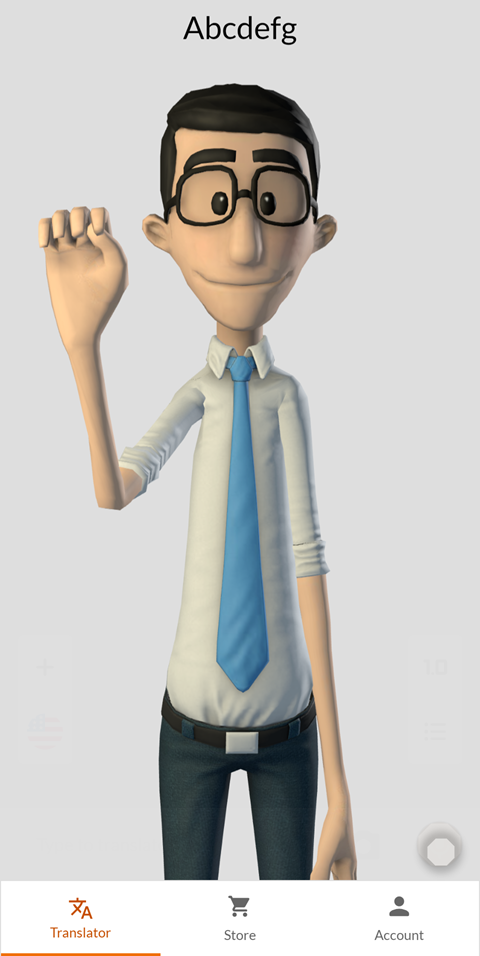
\includegraphics[width=0.25\columnwidth]{graphics/hand-talk-translator.png}
                    \caption{Aplikace Hand Talk Translator}
                    \label{hand-talk-translator}
                \end{figure}
                
            \item \emph{Znakujte s~Tamtamem} \par
                Povedená mobilní aplikace, která obsahuje základní znaky slov českého znakového jazyka. Znaky třídí do různých kategorií a~zobrazuje je pomocí videozáznamu, na kterém je člověk znakující daný znak. Aplikace umožňuje označovat znaky za již naučené a~pro procvičování nabízí kvízy, které jsou založeny na tom, že uživatel musí zvolit jednu ze tří odpovědí na základě zobrazeného znaku pomocí videa. \cite{tamtam}                

            \item \emph{Sign Language ASL Pocket Sign} \par
                Mobilní aplikace pro výuku amerického znakového jazyka. Také využívá videozáznamy pro zobrazování znaků. Navíc tyto videozáznamy dobře integruje do vzhledu aplikace, protože využívá záznamy s~vklíčovaným pozadím. Neumožňuje však volbu rychlosti přehrávání či ovládání úhlu pohledu. \cite{pocket-sign}
             
            \item \emph{www.spreadthesign.com} \par
                Webová stránka s~obsahem znaků slov a~písmen různých znakových jazyků, včetně českého. Obsahuje slovník s~videozáznamy. Vzhled stránky zobrazuje obrázek \ref{spread-the-sign.com}. \cite{spreadthesign}

            \begin{figure}[htbp]
                \centering
                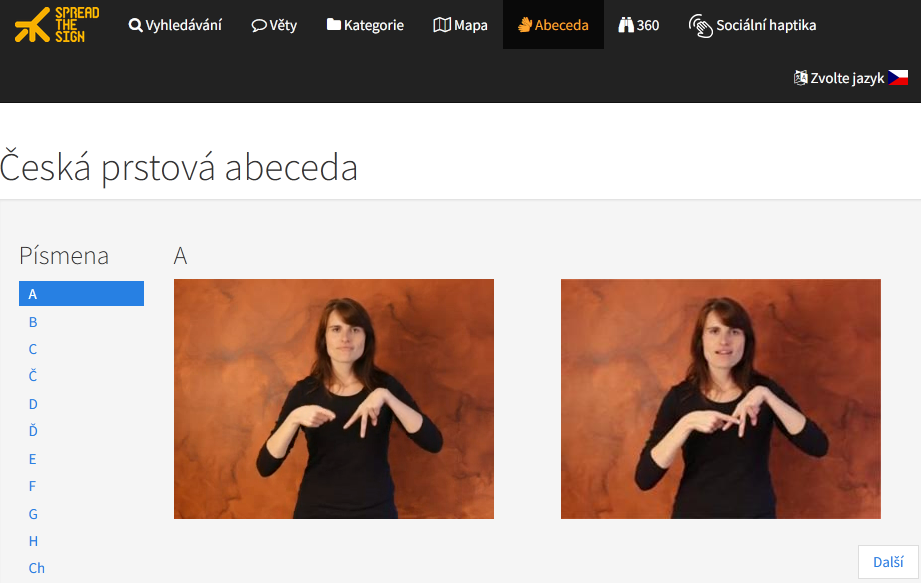
\includegraphics[width=0.8\columnwidth]{graphics/spread-the-sign.png}
                \caption{Webová stránka www.spreadthesign.com}
                \label{spread-the-sign.com}
            \end{figure}

             \item \emph{Webové stránky} \par
                Volně dostupné webové stránky s~obsahem o~jednoruční české prstové abecedě nebo i~o~ČZJ (český znakový jazyk) obsahují většinou pouze několik odstavců textu se statickým obrázkem obsahujícím jednotlivé znaky. Tyto stránky jsou většinou doprovázeny odkazy na placené kurzy.
                
            \item \emph{Mnoho dílčích projektů} \par
                Na internetu lze najít řadu malých projektů, které například implementují rozpoznání prstové abecedy z~webkamery, nicméně jsem nedohledal žádnou funkční aplikaci, která by podobnou funkcionalitu nabízela obzvlášť za účelem výuky či v~českém jazyce.
        \end{itemize}     


         Většina existujících řešení využívá videozáznamy pro ukázky znaků. Velkou výhodou při použití animací místo videozáznamů je flexibilita aplikace a~příjemnější vzhled. Animace například nabízí možnost změnit úhel pohledu nebo změnu rychlosti přehrávání bez ztráty plynulosti. 
         
         Žádné z~prozkoumaných řešení nenabízí funkci ověření správnosti znakování uživatelem pomocí rozpoznávání. Vyvinutá aplikace tedy přichází s~inovativním přístupem pomocí rozpoznání znaků z~webkamery a~tím nabízí nový přístup, jak se učit prstovou abecedu.

     \subsection{Funkcionalita aplikace}
       Tato podkapitola uvádí seznam všech požadavků na funkcionalitu a~chování vyvinuté aplikace. Tento seznam vychází zejména ze zadání práce, ale obsahuje i~aspekty, kterými byla aplikace rozšířena nad rámec zadání. Tento seznam slouží pro lepší představu o~vyvíjené aplikaci a~také k~sjednocení všech funkcionalit aplikace.

        \begin{itemize}
            \item Převod textu na plynulou sekvenci 3D animací interpretující daný text v~české jednoruční prstové abecedě.
            \begin{itemize}
                \item Možnost měnit rychlost přehrávání animace a~jejího zastavení.
                \item Možnost ovládání úhlu pohledu.
            \end{itemize}
            
            \item Rozpoznání zobrazeného znaku na snímku z~webkamery.
            
            \begin{itemize}
                \item Za účelem ověření, zda je zobrazen správný znak.
                \item Za účelem pokusu o~přepsání souvislé sekvence snímků do souvislého textu.
            \end{itemize}
            
            \item Různé režimy sloužící k~podpoře výuky a~procvičování české jednoruční prstové abecedy.
            
            \item Responzivní webová aplikace, kterou lze používat jak na velkých, tak i~malých obrazovkách.
            
            \item Možnost používání aplikace bez přístupu k~internetu.
            
            \item Možnost volby dvouruční české prstové abecedy a~českého znakového jazyka v~režimech nevyžadujících rozpoznávání znaků.
        \end{itemize}

\clearpage

\section{Znakový jazyk}
    Znakové jazyky představují plnohodnotné systémy, které slouží jako primární komunikační prostředek pro komunity neslyšících a~nedoslýchavých po celém světě. Na rozdíl od jazyků mluvených, které využívají zvuk, jsou znakové jazyky založeny na vizuální podobě. To znamená, že informace jsou předávány prostřednictvím kombinace tvarů rukou, jejich umístění a~pohybu v~prostoru, mimiky, pohybů hlavy a~horní části trupu. Je klíčové zdůraznit, že znakové jazyky nejsou pouhou pantomimou nebo manuální reprezentací mluvených jazyků; mají vlastní komplexní gramatiku, syntaxi a~bohatou slovní zásobu.


    Podobně jako mluvené jazyky, i~znakové jazyky vykazují značnou geografickou a~kulturní diverzitu. Neexistuje jeden univerzální znakový jazyk. Prakticky každý stát má svůj vlastní unikátní znakový jazyk (např. Český znakový jazyk – ČZJ, Americký znakový jazyk – ASL atd.), který se vyvíjel nezávisle. Tato rozmanitost se týká nejen samotných znaků pro slova a~pojmy, ale také systémů pro reprezentaci písmen – prstových abeced. \cite{ruce.cz}

\subsection{Prstová abeceda}

    Nedílnou součástí většiny znakových jazyků je prstová abeceda. Jedná se o~systém manuálních znaků (pozic ruky a~prstů), které vizuálně reprezentují jednotlivá písmena psané abecedy daného jazyka. Její primární funkcí není běžná komunikace, pro kterou slouží komplexní znaky reprezentující celé pojmy, ale spíše komunikace v~situacích, kdy pro daný pojem neexistuje ustálený znak, nebo je potřeba zdůraznit psanou podobu slova. Typické využití zahrnuje vlastní jména nebo odborné termíny.

    Prstové abecedy se celosvětově liší nejen tvary jednotlivých znaků pro písmena, ale také základním principem jejich provedení. Hlavní dělení je podle počtu rukou zapojených do znakování:

    \begin{itemize}
        \item \emph{Jednoruční prstové abecedy} \par
            K~vytvoření znaku pro písmeno se používá pouze jedna ruka (obvykle dominantní). Tvary ruky a~prstů se snaží stylizovaně napodobit tvar písmene.
        \item \emph{Dvouruční prstové abecedy} \par
            K~vytvoření znaku pro písmeno se používají obě ruce, které vzájemně spolupracují. Jedna ruka často tvoří základ tvaru a~druhá jej doplňuje, nebo ruce společně formují tvar písmene.
    \end{itemize}
    
    I~v~rámci jednoho typu mohou existovat drobné regionální či historické varianty jednotlivých znaků.

    \subsection{Prstové abecedy v~České republice}
    
        V~českém prostředí se setkáváme s~oběma hlavními typy prstových abeced – jednoruční i~dvouruční.
    
        \subsubsection{Česká jednoruční prstová abeceda}
        
            Tato diplomová práce a~výsledná aplikace se zaměřují specificky na podporu výuky české jednoruční prstové abecedy. Důvodem pro toto zaměření je, že pro slyšící začátečníky může představovat určitou výzvu. Ačkoliv se tvary ruky snaží vizuálně přiblížit podobě písmen, vyžadují poměrně vysokou míru přesnosti v~provedení a~pozici prstů. Některé znaky si mohou být pro nezkušené oko velmi podobné, což může zpočátku činit potíže při jejich rozlišování a~učení. 
        
        
            Vizualizaci všech znaků používaných v~české jednoruční prstové abecedě poskytuje obrázek \ref{prstova-abeceda}.
        
        \begin{figure}[htbp]
            \centering
            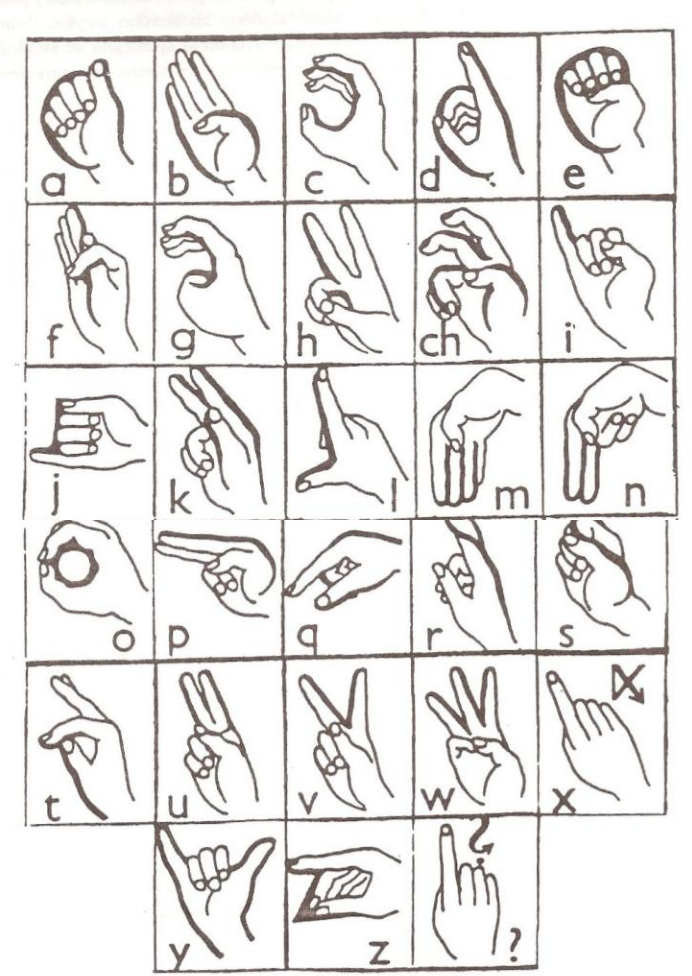
\includegraphics[width=0.5\columnwidth]{graphics/prstova-abeceda.png}
            \caption{Česká jednoruční prstová abeceda \cite{prstova-abeceda}}
            \label{prstova-abeceda}
        \end{figure}
        
        \subsubsection{Reprezentace diakritiky}
        
            Česká jednoruční prstová abeceda, stejně jako český jazyk, pracuje s~diakritickými znaménky (háčky a~čárky). Jejich reprezentace není řešena samostatným znakem, ale dynamickým pohybem ruky, který následuje po ukázání základního znaku písmene.
        
            \begin{itemize}
                \item Pro \emph{čárku} se po zobrazení znaku písmene provede krátký pohyb ruky shora dolů, vizuálně napodobující tvar čárky.
                \item Pro \emph{háček} se obdobně provede pohyb ruky naznačující tvar háčku (obvykle krátký pohyb šikmo dolů a~šikmo vzhůru).
            \end{itemize}
    
\clearpage



\section{Převod textu na animaci}
    Cílem této části je implementace převodu textu na 3D animaci, ve které bude postava ukazovat sekvenci znaků odpovídající danému textu s~možností volby rychlosti přehrávání animace.
    
    K~vytvoření takového systému je potřeba vytvořit 3D model postavy, vytvořit pro tento model animace konkrétních znaků a~následně tento model vykreslit a~řídit pomocí algoritmu posloupnost zobrazených animací znaků na vykresleném modelu. 
    Tento komplexní úkol je rozdělen do vhodných menších částí, které jsou popsány v~následujících podkapitolách.
    
    \subsection{Použité technologie}
        Jedinou použitou technologií při tvorbě animací na již vytvořeném 3D modelu postavy je Blender.
        
        \subsubsection{Blender}
            Blender je open-source software pro tvorbu 3D grafiky, který je zdarma dostupný pro všechny platformy. Tento program nabízí širokou škálu nástrojů pro modelování, texturování, animaci a~rendering 3D objektů. Blender je velmi populární mezi profesionály i~amatéry díky své flexibilitě a~rozsáhlé komunitě, která neustále přispívá k~jeho rozvoji. 
            Při vývoji aplikace sloužil Blender pro vytvoření animací znaků na již vytvořeném modelu člověka. \cite{blender}

      
    \subsection{Animování modelu}
        Prvním krokem je vytvoření 3D modelu postavy, který zobrazuje jednotlivé znaky v~podobě animací. Každý znak je reprezentován jednou animací, která je následně přehrávána v~sekvenci podle zadaného textu.

        \subsubsection{3D model člověka}
            Nejprve je potřeba vytvořit 3D model člověka. Takový model lze vytvořit například v~programu Blender. Vytvoření vizuálně zdařilého modelu postavy není triviální záležitost, z~tohoto důvodu byl použit již vytvořený model.

            Mixamo \cite{mixamo} je online platforma, kterou vlastní společnost Adobe. Poskytuje širokou škálu 3D modelů a~animací zdarma. Uživatelé mohou na Mixamo najít předem vytvořené 3D modely postav a~animace, které lze snadno integrovat do různých 3D projektů. Mixamo také umožňuje automatické rigování, což znamená, že uživatelé mohou nahrát své vlastní 3D modely a~Mixamo automaticky přidá kostru postavy, umožňující pohyb daného modelu. Tato platforma je velmi užitečná pro vývojáře her, animátory a~další profesionály pracující s~3D grafikou. Model postavy byl použit právě z~této platformy. 
            
    
        \subsubsection{Animace}
            Animování modelu je náročný proces. Zjednodušeně řečeno, vytvoření animace probíhá nejdříve pojmenováním animace, poté pomocí časové osy se v~konkrétních časech nastavují pozice a~rotace kostry modelu. Nastavení kostry ale není potřeba dělat pro každý snímek dané animace, chybějící snímky jsou automaticky dopočítávány.

            Manuální vytváření animací je velmi časově náročné, proto byla využita \emph{Pose Library}, která uchovává jedno konkrétní nastavení kostry. Jedno nastavení zastupuje výchozí stav, ze kterého všechny ostatní animace vycházejí, a~dále je pro každý znak vytvořeno jedno nastavení kostry reprezentující dané písmeno. 
            
            Výsledná animace je vytvořena tak, že se první snímek animace nastaví na výchozí pozici a~poslední snímek na pozici znaku. Animace je i~přesto velmi plynulá, jelikož jsou chybějící snímky dopočítávány. 
            
            Nicméně, při tomto jednoduchém přístupu mohou nastávat nežádoucí situace, kdy například prst projde jiným prstem. Tento problém by bylo možné vyřešit použitím více nastavení kostry v~průběhu animace. Ve výsledné aplikaci je tento problém řešen prolnutím animací do sebe (viz \ref{ovladani-animaci}), přičemž zmíněné situace nijak nenarušují dojem z~plynulosti a~správnosti animace.
           
        \subsubsection{Vytvoření animací pomocí aplikace Blender}
            V~této sekci je stručný popis funkcionalit, který popisuje proces tvorby animací. Prostředí aplikace při tvorbě animací je zobrazeno na obrázku \ref{blender}.

            \begin{itemize}
                    \item Model \par
                        Nejprve je potřeba vytvořit nebo nahrát již vytvořený model s~kostrou. Blender podporuje mnoho formátů 3D modelů, včetně formátu \emph{FBX}, který je podporován platformou Mixamo.
                        
                    \item Pozice \par
                        V~režimu \emph{Pose} je možné nastavovat pozice a~rotace jednotlivých kostí v~kostře modelu.
                        
                    \item Animace \par
                        Animace se vytváří pomocí \emph{Action Editor}, který obsahuje již zmíněnou časovou osu a~další nástroje pro vytváření animací. Průběh tvorby si lze představit tak, že se nastaví konkrétní čas na časové ose, zapne se tlačítko záznamu a~následně se nastaví pozice a~rotace kostí. Tím se dané nastavení kostry aplikuje v~daném čase animace. V~použitém případě se na konkrétní časové místo aplikuje kostra z~\emph{Pose Library}.
                        
                    \item Výraz obličeje \par
                        Ve znakovém jazyku je důležitý pohyb úst. Tento pohyb ale není možné zobrazit pomocí kostry, jelikož ústa a~obličej celkově nejsou součástí výchozí kostry. Tento problém je možné vyřešit například pomocí \emph{Shape keys}. Pomocí této techniky lze vytvářet jednoduché deformace modelu, které lze ovládat například pomocí pohybu nové kosti, kde se pozice kosti prováže s~hodnotou \emph{Shape key}. Poté lze upravovat výraz obličeje pomocí pozice konkrétních kostí jako u~výchozích kostí kostry.
                \end{itemize}

             \begin{figure}[htbp]
                \centering
                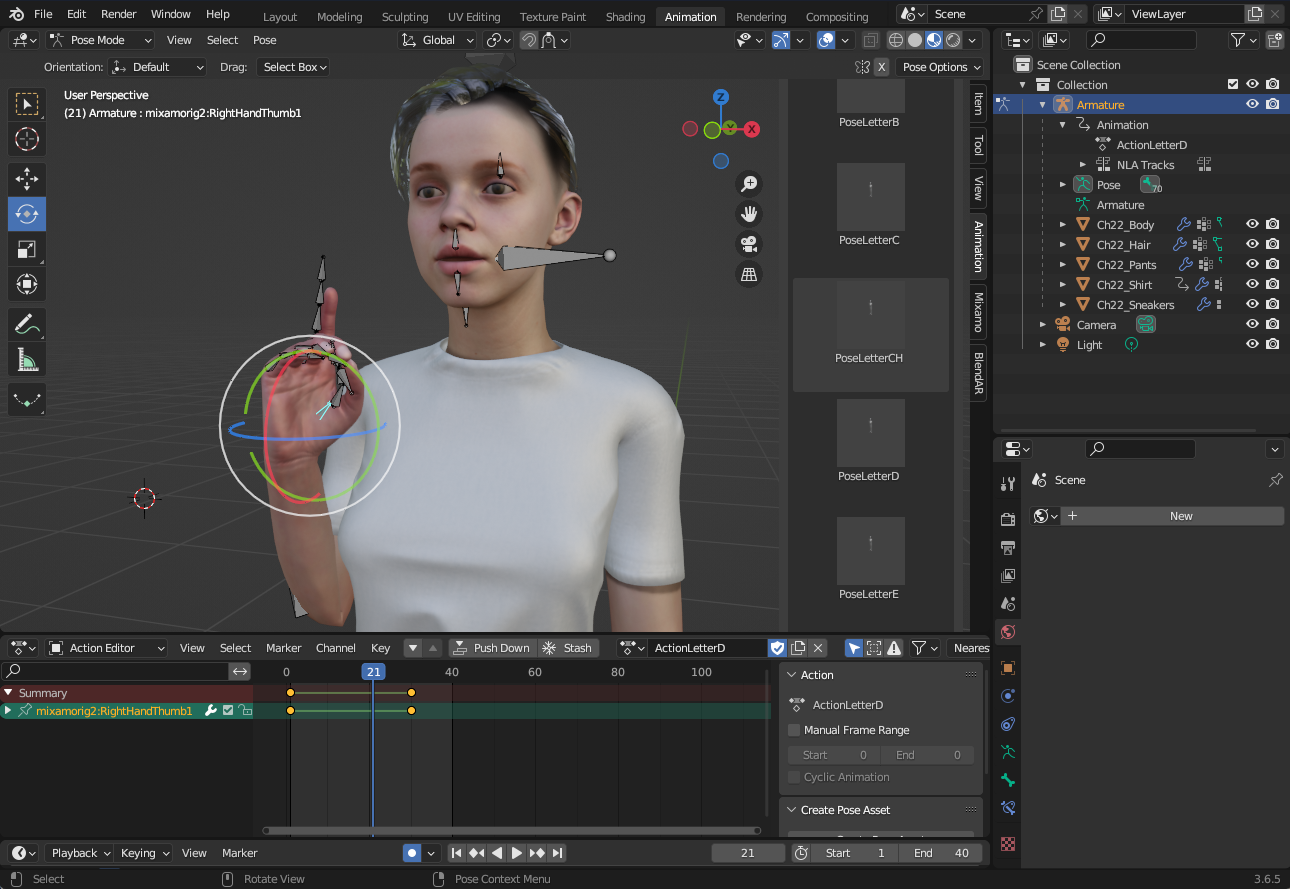
\includegraphics[width=1\columnwidth]{graphics/blender.png}
                \caption{Ukázka animování v~aplikaci Blender}
                \label{blender}
            \end{figure}
                
            \subsubsection{Exportování modelu}
                Pro použití modelu na webové stránce je klíčová jeho velikost. Použitý model při výchozím uložení obsahuje zhruba 100 MB dat ve formátu glb. Taková velikost je pro použití na webové stránce příliš velká, proto je potřeba model specificky exportovat, s~cílem minimalizovat jeho velikost. Model lze komprimovat dvěma hlavními způsoby. Komprimovat lze samotný 3D model pomocí Draco komprese, a~textury modelu lze komprimovat například převodem do .jpg formátu nebo zmenšením jejich rozlišení. Kombinací těchto dvou přístupů vznikl model s~velikostí kolem 10 MB.
    
    
    \subsection{Řízení přehrávání animací}
        Vytvořený model je potřeba nějakým způsobem zobrazit a~spouštět jeho animace ve správném pořadí a~načasování. V~této sekci je daný problém popsán obecně.

        Konkrétní vykreslení modelu a~řízení animací je popsáno v~kapitole Webová aplikace (kapitola \ref{webova-aplikace}), která využívá knihovnu Threlte spolu s~vytvořeným modelem z~této kapitoly.


        \subsubsection{Řídící algoritmus}
            Animace je potřeba přehrávat postupně za sebou. Tedy je nutné vstupní text rozložit na jednotlivé animace znaků. Pro každý jeden znak je potom spuštěna animace, která odpovídá danému znaku a~zvolenému jazyku. Je potřeba detekovat konec této animace a~na jejím konci spustit další animaci pro následující znak. Popsaný postup je opakován, dokud nejsou všechny znaky přehrány.

           K~přechodům jsou poté dodány prodlevy. Na konci každé animace je zobrazený znak na chvíli ponechán. Na konci celých slov je také vytvořena prodleva na signalizaci mezery mezi slovy.
        
        \subsubsection{Plynulý přechod mezi animacemi}
            Jelikož nejsou animace v~tomto případě příliš sofistikovaně vytvořeny a~nenavazují na sebe, tak je potřeba řídit jejich přechody tak, aby vypadaly přirozeně. Tento problém lze vyřešit splynutím konce aktuální animace do začátku následující animace.

        \subsubsection{Ovládací prvky}
            Důležitým aspektem a~výhodou přehrávání animací je volba její rychlosti. Tato funkcionalita je pro cílovou aplikaci velice vhodná. Začátečníci mohou používat aplikaci v~pomalejším tempu a~pokročilým uživatelům umožní využívat různé režimy ve vyšší rychlosti a~tím výrazně zvýšit náročnost procvičování. 
            
            Volba rychlosti také ovlivňuje délky prodlev, kde s~pomalejší rychlostí přehrávání časové rozmezí prodlev stoupá a~díky tomu se nenaruší plynulost celého přehrávání animace.

            Animaci lze v~průběhu zastavit a~znovu spustit. V~průběhu animace umožní tento ovládací prvek zastavení animace v~konkrétním bodě a~uživatel si poté může pohodlně prohlédnout zobrazený znak.

            Zmíněné zastavení se váže i~s~dalším ovládacím prvkem, který je umožněn díky vykreslení modelu ve 3D prostoru. To umožňuje pohybovat kamerou ve všech směrech a~tím si prohlédnout dané znaky z~jakéhokoliv úhlu a~pozice.

\clearpage



\section{Rozpoznání prstové abecedy z~videa}
    Následující problém je řádově složitější a~zajímavější než ten předchozí. Pokud bychom výše popsaný převod z~textu na animaci otočili a~vyměnili animaci za video z~reálného světa, tak se dostaneme k~následujícímu problému~--~převod české jednoruční prstové abecedy z~videozáznamu na text.

    Tento problém lze také rozdělit do několika podproblémů, konkrétně na rozpoznání souřadnic prstů ze snímku videozáznamu, zpracování těchto souřadnic, rozpoznání zobrazovaného znaku ze zpracovaných souřadnic a~převod všech rozpoznání na souvislý text. Při vytváření rozpoznávání narazíme ještě na jeden podproblém a~tím je dataset s~trénovacími daty.
        
    \subsection{Použité technologie}
        V~této podkapitole jsou popsány klíčové technologie, kterými je problém rozpoznání prstové abecedy z~videa řešen.
        
        \subsubsection{MediaPipe Solutions}
                Souhrn knihoven a~nástrojů od společností Google, které slouží k~různým rychlým nasazením metod umělé inteligence do aplikace. Nabízí podporu pro Android, iOS, JavaScript a~Python. MediaPipe již obsahuje několik hotových, v~některých případech rozšiřitelných, řešení například pro rozpoznání obličeje, objektovou klasifikaci, text embedding a~zejména rozpoznání orientačních bodů (souřadnic) ruky. Poslední zmíněné řešení je klíčovou součástí vyvinuté aplikace a~její použití značně zjednodušilo vývoj a~umožnilo vysokou přesnost tohoto systému. \cite{mediapipe}
                
        \subsubsection{TensorFlow}
                TensorFlow je open-source knihovna pro strojové učení vyvinutá společností Google. Je velmi populární mezi vývojáři díky své flexibilitě a~široké škále nástrojů pro vytváření a~trénování modelů strojového učení. TensorFlow je dostupný pro všechny hlavní platformy a~podporuje mnoho programovacích jazyků, včetně Pythonu a~JavaScriptu. TensorFlow je použit pro vytvoření modelu pro rozpoznání prstové abecedy. \cite{tensorflow}
                
        \subsubsection{TensorFlow Decision Forests}
                TensorFlow Decision Forests (zkráceně TFDF) je knihovna pro TensorFlow, která poskytuje nástroje pro vytváření a~trénování rozhodovacích lesů. Rozhodovací lesy jsou populární metodou strojového učení, která se používá pro klasifikaci a~regresi dat. TFDF je použit pro vytvoření modelu pro rozpoznání prstové abecedy. \cite{tensorflow-tfdf}

       \subsubsection{Gradient Boosted Trees}
            Gradient Boosted Trees (GBT) je výkonná metoda strojového učení založená na vícero rozhodovacích stromech. Pracuje iterativně, přičemž se každý nový strom učí opravovat chyby předchozích stromů minimalizací gradientu ztrátové funkce. GBT je široce používán pro klasifikaci i~regresi díky své schopnosti efektivně zachytit složité vzory v~datech. Populární knihovny implementující GBT zahrnují XGBoost, LightGBM a~TensorFlow Decision Forests. \cite{gbdt}
                
        \subsubsection{Python}
                Python je všeobecný programovací jazyk, který je velmi populární mezi vývojáři díky své jednoduché syntaxi a~široké škále knihoven a~nástrojů pro různé účely. Python je použit pro tvorbu skriptů, které vedou k~vytvoření modelu pro rozpoznání prstové abecedy.

    
    \subsection{Proces rozpoznání gest}
        Rozpoznání zobrazeného znaku ze snímku kamery probíhá následujícími kroky.

        \begin{enumerate}
            \item Rozpoznání pozice ruky a~prstů
            \item Zpracování rozpoznaných dat
            \item Klasifikace zpracovaných dat
        \end{enumerate}

        Všechny zdrojové kódy sloužící k~tvorbě modelu pro rozpoznávání gest se nacházejí ve složce \emph{python\_recognition}. Diagram zobrazující tok dat mezi jednotlivými částmi při tvorbě klasifikátoru lze vidět na obrázku \ref{python-training-flow-diagram}.

        \begin{figure}[htbp]
            \centering
            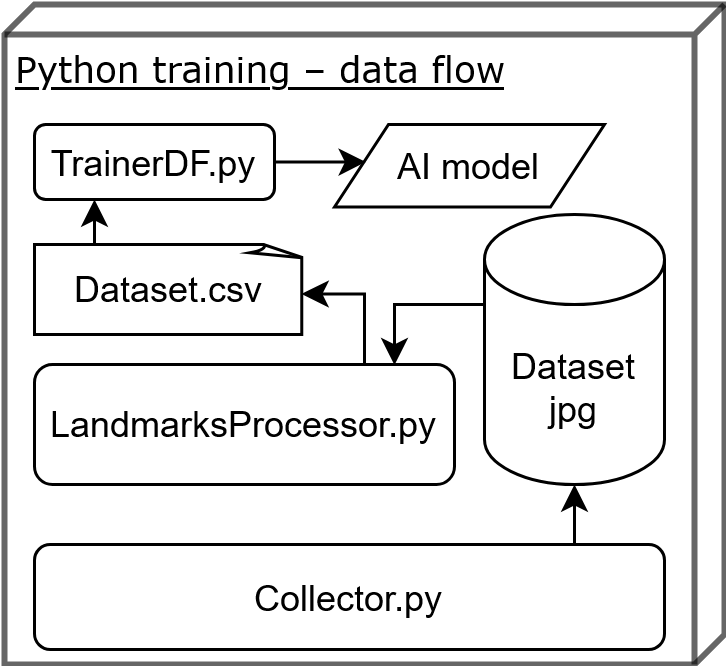
\includegraphics[width=0.5\columnwidth]{graphics/python-training-flow-diagram.png}
            \caption{Diagram toku dat při vytváření klasifikátoru}
            \label{python-training-flow-diagram}
        \end{figure}
        
        \subsubsection{Extrakce souřadnic bodů ruky}
           Pomocí modelu Hand Landmark Detection z~frameworku MediaPipe lze získat z~obrazu ruky 21 souřadnic, které reprezentují orientační body ruky. Tyto souřadnice jsou vyjádřeny trojicí $(x, y, z)$, kde $x$ a~$y$ jsou souřadnice bodů relativně k~celému snímku a~$z$~je vzdálenost od kamery.

           Velkou výhodou využití MediaPipe Hand Landmark Detection je vysoká přesnost určení souřadnic bodů ruky, a~to i~za špatných světelných podmínek, při různých rotacích ruky nebo při jakémkoliv pozadí, před kterým uživatel svou ruku zobrazuje. Názorné rozpoznání souřadnic lze vidět na obrázku \ref{mediapipe}.
           
           Tento fakt umožňuje se více zaměřit na klasifikaci rozpoznaných souřadnic a~tím se abstrahovat od problému správné detekce bodů ruky a~prstů.

         \begin{figure}[htbp]
            \centering
            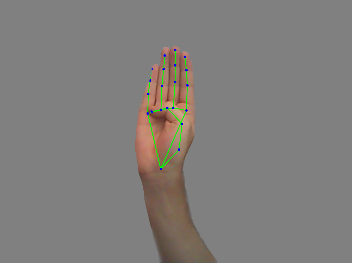
\includegraphics[width=0.5\columnwidth]{graphics/mediapipe.png}
            \caption{Rozpoznání 21 souřadnic ruky pomocí MediaPipe Solutions}
            \label{mediapipe}
        \end{figure}
           

        \subsubsection{Zpracování souřadnic} \label{zpracovani-souradnic}
            Pro efektivní zpracování souřadnic metodami strojového učení je potřeba souřadnice převést do vhodného formátu. Aplikace souřadnice nejprve převede tak, aby byly reprezentovány relativně k~souřadnici pozice zápěstí (souřadnice s~indexem 0) a~tím zanikne závislost na pozici ruky v~určité části snímku kamery. Následně jsou souřadnice normalizovány do rozsahu $[-1, 1]$ a~tím zaniká závislost na vzdálenosti ruky od kamery. 

              Algoritmus zpracovává souřadnice \emph{x} a~\emph{y}, hodnota \emph{z} je ignorována. Tím je výsledný klasifikátor značně zjednodušen. Model s~menší dimenzionalitou vyžaduje méně dat při učení a~snižuje se riziko přeučení modelu při použití malého datasetu. Hodnota \emph{z} je také méně spolehlivá/přesná a~z~těchto důvodů je ignorována, ačkoliv by poskytovala další informaci o~zobrazeném gestu ruky. 
          
          Tento postup vychází z~již existujícího řešení tvorby klasifikátoru gest ruky \cite{mediapipe-example}.
           
        \subsubsection{Klasifikace}
            Klasifikace je metoda, která na vstupu přijímá zpracované souřadnice prstů ruky a~na základě těchto souřadnic vyhodnocuje, s~jakou pravděpodobností je jaký znak vyobrazen.
            
    
    \subsection{Tvorba klasifikátoru}
        Při vytváření klasifikátoru je nejdůležitější mít dataset obsahující data, na kterých bude model trénován. Nad takovými daty je poté spuštěn trénovací algoritmus, jehož výstupem je model, který lze použít pro klasifikaci souřadnic ruky.

        \subsubsection{Dataset}
            Datasetem jsou v~tomto případě fotky, na kterých je viditelná ruka člověka zobrazující nějaký konkrétní znak. Tyto fotky jsou v~jednotlivých složkách, kde každá složka obsahuje fotky s~jedním konkrétním znakem. Velikost datasetu je zhruba 100 fotek jedné osoby a~25 fotek druhé osoby na každý znak české jednoruční prstové abecedy pro levou i~pravou ruku. K~těmto znakům je ještě přidán znak \emph{None}, reprezentující žádný znak za účelem zpřesnění klasifikace. Dohromady dataset obsahuje 7217 snímků v~rozlišení 250x250 pixelů. Strukturu a~ukázku obrázků datasetu zobrazuje obrázek \ref{dataset}.

            Každý snímek je převeden do formátu zpracovaných souřadnic a~uložen do .csv souboru, který je použit jako vstup pro trénovací algoritmus. Během tohoto zpracování jsou data dále rozšířena pomocí techniky známé jako \emph{augmentace dat}. Jejím principem je umělé navýšení objemu trénovacích dat pomocí provedení různých změn nad již existujícími daty. V~tomto případě bylo využito horizontálního zrcadlení každého snímku. Tato transformace je zde vhodná, protože zrcadlový obraz znaku zobrazeného levou rukou vizuálně odpovídá stejnému znaku zobrazenému pravou rukou a~naopak. Pro téměř každý původní snímek tak vznikají dva záznamy zpracovaných souřadnic, čímž se velikost trénovacího datasetu téměř zdvojnásobí.

            K~tvorbě datasetu existují dva skripty v~jazyce Python ulehčující tento proces. Prvním je \emph{Collector.py}, který v~okně zobrazí záznam webkamery a~odposlouchává stisky kláves klávesnice. Pokud uživatel stiskne písmeno na klávesnici, tak se algoritmus pokusí získat souřadnice prstů ruky z~bufferu několika posledních snímků kamery. Nejnovější ořezaný snímek, ze kterého lze rozeznat souřadnice prstů ruky, se uloží do složky s~názvem odpovídajícím stisknuté klávesy. 
            
            Druhým skriptem je \emph{LandmarksProcessor.py}, který zpracuje všechny snímky v~dané struktuře složek a~uloží je do .csv souboru.


         \begin{figure}[H]
            \centering
            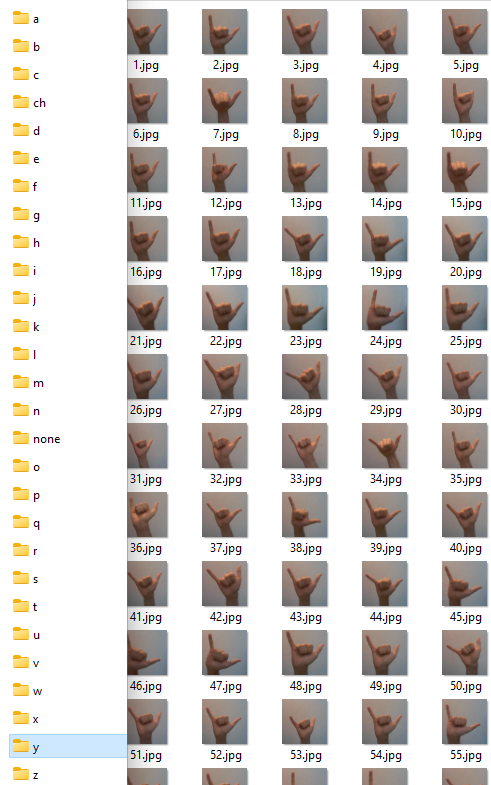
\includegraphics[width=0.55\columnwidth]{graphics/dataset.png}
            \caption{Ukázka datasetu písmene Y}
            \label{dataset}
        \end{figure}
           

        \subsubsection{Použití frameworku MediaPipe v~Pythonu}
        Ukázka použití MediaPipe Solutions frameworku, konkrétně Hand Landmark Detection v~jazyce Python viz zdrojový kód \ref{mediapipe-python}.
        
        \begin{kicode}{Python}{mediapipe-python}{Použití MediaPipe Solutions v~Pythonu}
import mediapipe as mp
import cv2

# Načtení obrázku
image = cv2.imread(file_path)

hands = mp.solutions.hands.Hands(
    static_image_mode=STATIC_IMAGE_MODE,
    max_num_hands=MAX_NUM_HANDS,
    min_detection_confidence=MIN_DETECTION_CONFIDENCE,
    min_tracking_confidence=MIN_TRACKING_CONFIDENCE,
)

result = hands.process(image)
        \end{kicode}
        
        \subsubsection{Trénování sítě}
           Pro~žádanou klasifikaci souřadnic existuje spousta metod, v~rámci této práce byly vyzkoušeny následující metody:

           \begin{itemize}
                \item MediaPipe Gesture recognition
                \item Neuronové sítě
                \item XGBoost
                \item TensorFlow Decision Forests~--~Gradient Boosted Trees.
            \end{itemize}

        MediaPipe Gesture recognition nabízí možnost úpravy a~rozšíření jejich modelu pro rozpoznávání gest, který pracuje mírně odlišným způsobem při zpracování souřadnic oproti ostatním vyzkoušeným přístupům. Nejprve z~extrahovaných souřadnic vytvoří 128 prvkový vektor pomocí neuronové sítě a~následně daný výsledek embeddingu klasifikuje další neuronovou sítí. Tato metoda měla mírně vyšší přesnost než vlastní implementace neuronových sítí se zmíněným zpracováním souřadnic z~podkapitoly \ref{zpracovani-souradnic}.
    
       Ve finální aplikaci je použita metoda \emph{Gradient Boosted Trees} z~knihovny TensorFlow Decision Forests. Oproti neuronovým sítím měla tato metoda výrazně větší přesnost. Metoda XGBoost byla mírně přesnější než TFDF Gradient Boosted Trees, ale ve finální aplikaci nebyla použita z~důvodu náročnosti integrace do webové aplikace. 
        
        K~trénování modelu slouží skript \emph{TrainerDF.py}, který rozdělí vstupní data z~.csv souboru do trénovací a~testovací množiny. Poté nad trénovací množinou spustí trénovací algoritmus poskytnutý knihovnou TensorFlow Decision Forests a~následně natrénovaný model vyhodnotí a~uloží do formátu, který je využíván knihovnou TensorFlow v~JavaScriptu.


        \subsubsection{Použití TensorFlow v~Pythonu}
            Ukázka použití TensorFlow knihovny v~jazyce Python. Následující zdrojový kód \ref{tfdf-python} ukazuje příklad trénování \emph{Gradient Boosted Trees} modelu. 
                 
                 \begin{kicode}{Python}{tfdf-python}{Použití TensorFlow Decision Forests v~Pythonu}
import tensorflow_decision_forests as tfdf

# Příprava rozdělených dat
train_ds = tfdf.keras.pd_dataframe_to_tf_dataset(train_set, label="label")
test_ds = tfdf.keras.pd_dataframe_to_tf_dataset(test_set, label="label")

# Vytvoření klasifikátoru
model = tfdf.keras.GradientBoostedTreesModel(verbose=2)
model.fit(train_ds)

# Evaluace modelu
model.compile(metrics=["accuracy"])
evaluation = model.evaluate(test_ds, return_dict=True)

# Uložení modelu
model.save(OUTPUT_TFDF_MODEL_PATH)
tfjs.converters.tf_saved_model_conversion_v2.convert_tf_saved_model(OUTPUT_TFDF_MODEL_PATH, OUTPUT_TFJS_MODEL_PATH)
                \end{kicode}


        \subsubsection{Přesnost modelu}
            Natrénovaný model má přesnost \(\sim \)96~\% na testovací množině dat. Při testování neuronových sítí se přesnost pohybovala zhruba o~\(\sim \)10~\% níže. Důležitým faktorem pro reálné použití modelu je přesnost pro každý znak zvlášť. Pokud by model vyhodnocoval všechny znaky kromě jednoho správně a~ten jeden zcela špatně, tak by byl takový model v~aplikaci nepoužitelný. Pro takové vyhodnocení lze využít například matici záměn. Tabulku reprezentující takovou matici lze vidět na obrázku \ref{confusion-matrix}, která obsahuje hodnoty použitého modelu.

             \begin{figure}[htbp]
                \centering
                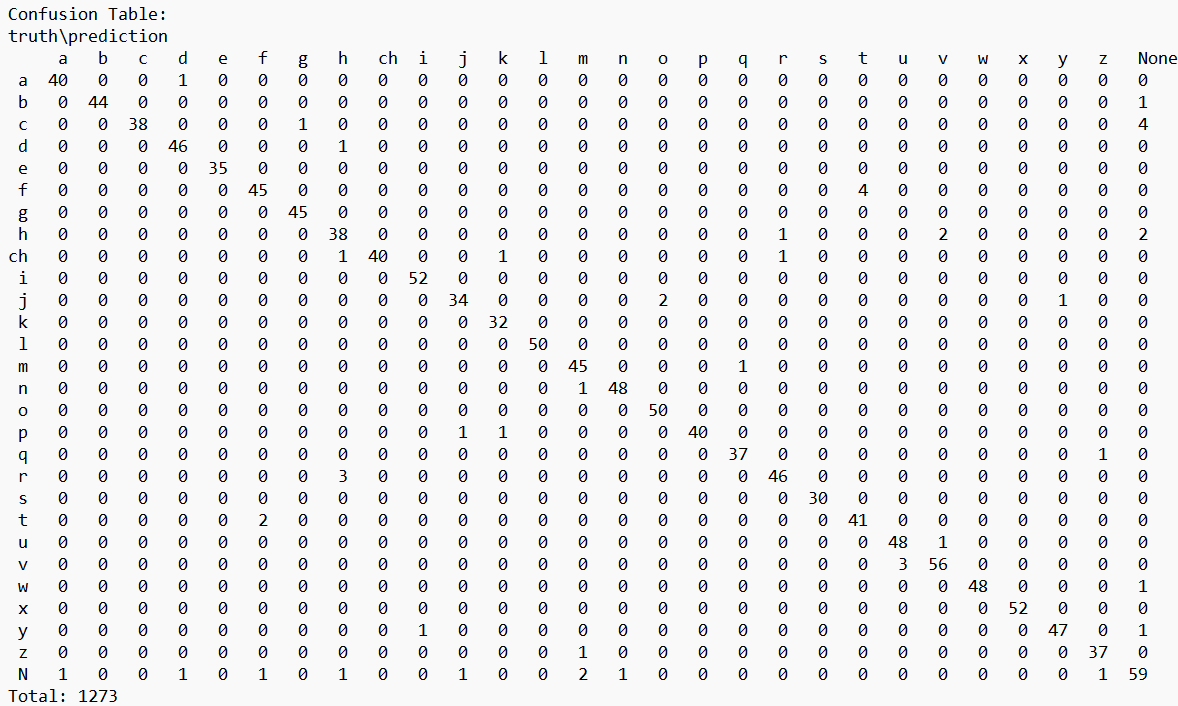
\includegraphics[width=0.9\columnwidth]{graphics/confusion-matrix.png}
                \caption{Matice záměn natrénovaného modelu}
                \label{confusion-matrix}
            \end{figure}
            
            Výsledná přesnost je mírně nižší (zhruba o~\(\sim \)2~\%) oproti článku \cite{benchmark-article}, který prezentuje GBT a~MediaPipe Solutions pro rozpoznání prstové abecedy ASL na zhruba 100\(\times\) větším datasetu. Menší přesnost je očekávaná na základě jednodušší práce se zpracováním souřadnic. Pro účely aplikace je natrénovaný model dostačující, ale nabízí se zde určitá vylepšení. Například ve zmíněné sofistikovanější práci se souřadnicemi ruky nebo využitím zcela jiného klasifikačního modelu. 
            
            Použitá metoda byla zvolena zejména na základě její jednoduchosti. Vytvořený model naplňuje očekávání pro funkcionalitu aplikace, jeví se jako schopný rozeznávat správně znaky a~tím kontrolovat uživatele. Model je také dostatečný pro převod videozáznamu na souvislý text.

            Je ale třeba podotknout, že model byl vytvořen na základě omezeného datasetu. Dataset obsahuje pouze dvě osoby a~tím může negativně přispět ke~schopnosti generalizace daného modelu. Model se mohl naučit specifika těchto dvou osob a~tím značně omezit schopnost rozeznávat gesta ruky osob jiných. Zmíněná přesnost modelu je počítána z~části vytvořeného datasetu a~při klasifikaci jiných osob bude zcela určitě nižší.


        \subsubsection{Převod modelu na tfjs}
            K~použití TensorFlow modelu na straně webového prohlížeče je nutné převést daný model do formátu, který je používán knihovnou TensorFlow.js. Ukázkový převod lze vidět ve zdrojovém kódu \ref{tfdf-python} na posledním řádku.
         
            
    
   \subsection{Problém určení času zápisu} \label{cslr-text}
        Výše popsanými metodami lze tedy rozpoznat znak z~jednoho snímku. K~plynulému rozpoznání slov či vět je potřeba nějakým způsobem určit, kdy je znak zobrazen a~kdy jej zaznamenat. S~tímto problémem se lze často setkat v~doméně rozpoznání znakové řeči pod zkratkou \emph{CSLR}~--~Continuous sign language recognition. Tento problém velmi komplikuje nedokonalost klasifikátoru, která místo reálně zobrazovaného znaku může rozeznat znak jiný.

        \subsubsection{Možná řešení}
            Možné přístupy k~řešení tohoto problému jsou:
            \begin{itemize}
                \item Získání potvrzení ze třetí strany, například stiskem klávesy na klávesnici či zobrazením speciálního gesta signalizujícího zápis minulého znaku nebo mezeru.
                \item Časová prodleva -- daný znak se považuje za zapsaný, pokud jej uživatel zobrazí po určitou dobu.
                \item Detekce pohybu ruky, změny znaku, například při výrazné a~rychlé změně pixelů obrazu.
            \end{itemize}


    \subsubsection{Popis použitého algoritmu}
        Výsledná aplikace implementuje pro přepis sekvence znakování na text jednoduchý heuristický přístup. Tento přístup s~sebou nese některá omezení. Vyžaduje relativně stabilní rychlost znakování a~specifické akce uživatele pro vložení mezery nebo pro zapsání zdvojených písmen.

        Algoritmus pracuje s~řetězcem znaků, který vzniká postupným přidáváním vždy nejpravděpodobnějšího znaku rozpoznaného v~jednotlivých snímcích z~webkamery s~určitou frekvencí. Tato frekvence je určena konstantou \emph{msToNextPredict} v~komponentě \emph{GestureRecognition} a~zásadně ovlivňuje očekávanou rychlost znakování uživatele. Samotný převod zmíněného řetězce všech rozpoznání na výsledný text zajišťuje funkce \emph{convertRecognitionsToText(input)} implementovaná v~souboru \emph{CSLR.ts}.

        Základem algoritmu je zpracování vstupního řetězce a~jeho převedení na výstupní text na základě frekvence výskytu znaků a~předdefinovaných prahových hodnot.
        
        \begin{itemize}
            \item \emph{MIN\_GROUP\_LENGTH} (výchozí hodnota 6): \\ Minimální počet po sobě jdoucích (nebo téměř po sobě jdoucích) výskytů stejného znaku, aby byl považován za platně zobrazený.
            \item \emph{SPACE\_INSERT\_THRESHOLD} (výchozí hodnota 20): \\ Práh počtu výskytů, při jehož překročení se za zapsaný znak přidá mezera.
            \item \emph{ERROR\_CONTEXT\_SIZE} (výchozí hodnota 1): \\ Počet znaků kolem potenciální chyby v~rozpoznávání, která se kontroluje pro možnost ignorování této chyby.
            \item \emph{MULTI\_CHAR\_TOKENS} (obsahuje 'Ch'): \\ Definuje vícepísmenné znaky, které se mají zpracovávat jako jeden celek.
        \end{itemize}
        
        Těchto pět konstant nepřímo určuje toleranci algoritmu a~očekávanou rychlost znakování. Výchozí nastavení je cíleno na začátečníky s~prstovou abecedou, což znamená pomalejší tempo, než jakým by znakoval zkušený uživatel. Možným vylepšením by mohla být dynamická úprava těchto konstant podle rychlosti uživatele.

        Konkrétní postup funkce \emph{convertRecognitionsToText}:

        \begin{enumerate}
            \item 
            Tokenizace: Vstupní řetězec je nejprve rozdělen na jednotlivé tokeny – znaky, přičemž se bere ohled na vícepísmenné znaky definované v~konstantě.
            
            \item 
            Iterace: Algoritmus prochází sekvenci tokenů a~počítá, kolikrát se aktuálně sledovaný token opakuje za sebou.
           
            \item 
            Tolerance chyb: Při kontrole opakování se uplatňuje tolerance vůči chybám. Pokud se objeví odlišný token, ale token před ním i~za ním vzdálen o~\emph{ERROR\_CONTEXT\_SIZE} pozic odpovídá aktuálně sledovanému tokenu, je daný token ignorován a~sekvence se považuje za nepřerušenou.
           
            \item 
            Registrace znaku: Jakmile sekvence aktuálního tokenu skončí a~objeví se jiný token, který nelze ignorovat dle pravidla tolerance chyb, nebo nastane konec vstupu. Tak algoritmus zkontroluje počet nasbíraných výskytů \emph{count}.
                \begin{itemize}
                    \item 
                        Pokud \emph{count} dosáhne alespoň \emph{MIN\_GROUP\_LENGTH} (6), token je považován za platný znak a~přidá se do výsledného textu.
                     \item 
                        Výjimka: Pro tokeny 'g'~a~'f'~stačí poloviční počet výskytů.
                    \item 
                        Vložení mezery: Pokud \emph{count} dosáhl nejen prahu pro registraci znaku, ale i~vyššího prahu \emph{SPACE\_INSERT\_THRESHOLD} (20), je stav interpretován jako signál konce slova a~za právě přidaný znak se do výsledku vloží mezera.
                \end{itemize}
            
            \item 
            Pokračování: Pokud vstupní sekvence ještě neskončila, nastaví se nový aktuální token a~proces pokračuje další iterací v~kroku 2.
        \end{enumerate}

    Znaky 'g'~a~'f'~vyžadují pouze polovinu rozpoznání, protože jsou častěji zaměňovány s~jinými znaky než ostatní písmena. Písmeno 'f' je zaměňováno s~písmenem 't'. Písmeno 'g' je zaměňováno s~písmeny 'c' a~'o'. K~těmto jednostranným záměnám dochází z~důvodu nedokonalosti rozpoznávání a~velké podobnosti zmíněných znaků písmen. Zmíněné podobnosti ale nejsou jedinými a~i~ostatní znaky písmen mají často velmi podobné znaky.


   \subsubsection{Příklad vstupu a~výstupu}
   
   \def\enablehyph#1{\enablehyphA #1\end}
\def\enablehyphA#1{\ifx\end#1\unskip\unpenalty
   \else#1\penalty0\hskip0pt plus1pt\relax
   \expandafter\enablehyphA\fi}

    Z~rozpoznaného řetězce písmen:\\ \emph{\enablehyph{
    MMMMMMMMMMMMAAASAAAAAAAAMMMMMMMMMMMMMMMMMMMMMMMMMMMMMMMMNZZKKKKKKKKKKKChOOOOOOCCCCCCCCCCCDChKKKKKKKKKKKKKChChUUUUUUUUUUUUUUUUUUUUUUUUUUSSSSSSSSSSSSSSSSSSSSSSEOEEEEEEERRRRRRRRRRRRRAAAAChRRRRRRRRRRRROOOOOOOOOHRRRRRRRRRRRRREEEEEEEEEEEOOMMMMMMMMMMMMMM
        }}\\ zmíněný algoritmus vyhodnotí skutečnou sekvenci znaků na skutečně zobrazené slovní spojení: \emph{MAM KOCKU S~ERROREM}.

        V~příkladě lze vidět, že vstup obsahuje necílené znaky při změnách skutečně zobrazovaných znaků (např. změna znaku z~písmene 'm' na písmeno 'k'~--~MMMMMMNZZKKKK). Tyto krátké sekvence nejsou ale rozpoznávány. 
        
        Také si lze všimnout ignorování osamělých znaků v~rámci některé sekvence (např.~zobrazené písmeno 'a' bylo nechtěně rozpoznáno jako písmeno 's'~--~AAASAAA).

        Algoritmus vyhodnocuje zdvojená písmena krátkým přerušením sekvence rozpoznání stejného znaku (např. rozpoznaného vstupu při znakování sekvence 'rr'~--~...RRRRAAAAChRRRRR...). Uživatel v~takový moment musí krátce zobrazit jiný znak~--~přerušit ukazování zdvojeného znaku a~tím dojde k~rozpoznání jiného znaku.

        U~posledních písmen ve slově lze vidět podstatně delší sekvenci rozpoznání.

    \subsubsection{Propojení s~LLM}
        Proces rozpoznání záznamu kamery na souvislý text je náročný a~zcela určitě bude docházet k~chybám. Tím se nabízí problém, jak detekovat tyto chyby a~jak je opravit.

        Jedno z~tradičních řešení je například vytvoření databáze všech možných slov, kde by algoritmus měl za cíl pro slovo s~chybou najít takové slovo, kterému se nejvíce podobá. Jak už bylo zmíněno, některé znaky jsou zaměňovány častěji než jiné, tedy do tohoto algoritmu by bylo možné zakomponovat výběr chtěného slova na základě toho, s~jakou pravděpodobností byl chybně rozpoznaný znak zaměněn za jiný.

        Implementace takového algoritmu ale není rozhodně přímočará a~zcela nefunkční pro slova, která by nebyla v~databázi slov. Zajímavým zamyšlením také je, že pravděpodobnost výskytu slova ve větě je provázána s~okolními slovy v~dané větě a~i~v~okolních větách~--~tedy s~kontextem celého textu. Tato úvaha, která v~posledních pár letech zcela změnila svět, mě přivedla na použití řešení tohoto problému pomocí velkých jazykových modelů (LLM).
        
        Výstup popsaného algoritmu \emph{CSLR} je možné provázat se vstupem velkého jazykového modelu. Vlastností takových modelů je porozumění kontextu slov v~textovém vstupu a~tím vzniklá schopnost zanedbání drobných chyb či překlepů takového vstupu.

        Zmíněné provázání \emph{CSLR} algoritmu s~velkým jazykovým modelem je využito v~režimu \emph{Konverzace}, který je popsán v~podkapitole \ref{up-konverzace}.


\clearpage


\section{Webová aplikace} \label{webova-aplikace}
    Spojením výše popsaných dvou částí vznikla webová aplikace, jejímž cílem je podpora výuky a~procvičování české jednoruční prstové abecedy. Aplikace rozšiřuje své funkcionality i~pro dvouruční českou prstovou abecedu a~nabízí podporu procvičování znaků českého znakového jazyka.

    \subsection{Použité technologie}
        V~této sekci jsou popsány technologie, na kterých je založena vyvinutá webová aplikace.
        
        \subsubsection{SvelteKit}
            SvelteKit je moderní framework pro vývoj webových aplikací. SvelteKit je založen na UI frameworku Svelte, který umožňuje jednoduchou tvorbu komponent, které jsou překládány do JavaScriptu a~efektivně vykreslovány v~prohlížeči. \cite{svelte}
    
        \subsubsection{Flowbite Svelte}
            Flowbite Svelte je open-source knihovna UI komponent pro Svelte. Poskytuje sadu předpřipravených komponent, které urychlují vývoj uživatelského rozhraní. Komponenty jsou optimalizované pro responzivní design a~umožňují rychlé vytváření konzistentního vzhledu aplikace. \cite{flowbite}
        
        \subsubsection{Tailwind CSS}
            Tailwind CSS je utility-first CSS framework, který umožňuje rychlé a~flexibilní stylování webových aplikací. Místo předpřipravených komponent používá nízkoúrovňové utility třídy. \cite{tailwind}
    
          \subsubsection{Three.js a~Threlte}
            Three.js je populární knihovna pro vytváření a~manipulaci s~3D grafikou v~prostředí webových prohlížečů pomocí JavaScriptu. Umožňuje snadné vytváření složitých 3D scén, animací a~interakcí. \cite{threejs} Threlte je nadstavba nad Three.js, která integruje tuto knihovnu do frameworku Svelte. Threlte poskytuje komponenty a~nástroje, které zjednodušují vytváření a~správu 3D scén a~animací ve Svelte aplikacích. 
            Threlte je použito ve vytvořené aplikaci pro zobrazení modelu postavy a~jeho animací. \cite{threlte}
        
        \subsubsection{TensorFlow.js}
            TensorFlow.js je knihovna pro strojové učení v~JavaScriptu, která umožňuje spouštění natrénovaných modelů ve webovém prohlížeči.

    \subsection{Architektura aplikace}
        Architektura webové aplikace je založena na komponentách, kde komponenta je ucelená nezávislá funkcionalita. Tyto komponenty lze vkládat do jiných komponent a~tím vytvořit komplexní strukturu, ve které je přehledně rozdělena zodpovědnost a~závislost pomocí domluvených rozhraní. 

        Hlavními prvky aplikace jsou stránky, mezi kterými se uživatel přepíná pomocí směrování. Tyto stránky definují vlastní obsah, který se většinou skládá z~kombinace zmíněných komponent. Stránka je zodpovědná za komunikaci mezi komponentami umístěnými uvnitř ní.

         \subsubsection{Struktura projektu}
            Struktura celého projektu se skládá z~následujících adresářů.

            \begin{itemize}
                \item \emph{/} \par
                    Kořenový adresář obsahující konfigurační soubory a~soubor \emph{package.json} definující závislosti webové aplikace.
                    
                \item \emph{/src} \par
                    Adresář obsahující zdrojové kódy webové aplikace. Obsahuje dva podadresáře a~soubory, které obalují celou aplikaci.
                    \begin{itemize}
                        \item \emph{/src/lib} \par
                            Adresář obsahující všechny komponenty aplikace a~soubory s~modely a~pomocnými funkcemi pro práci s~textem, inferencí AI modelů, zpracováním souřadnic a~CSLR vyhodnocením.
                        \item \emph{/src/routes} \par
                            Adresář obsahující soubory jednotlivých stránek a~soubory definující celkový layout aplikace. Adresářová struktura tohoto adresáře definuje směrování aplikace.
                    \end{itemize}
                    
                \item \emph{/static} \par
                    Adresář obsahuje všechny statické soubory webové aplikace. Nachází se zde ikony, manifest, AI modely, 3D model, seznam slov a~wasm soubory.

                \item \emph{/3D} \par
                    Adresář s~3D modelem.
                    
                \item \emph{/python\_recognition} \par
                   Adresář obsahující dataset a~zdrojové kódy použité při tvorbě klasifikačního modelu.
            \end{itemize}
         
        \subsubsection{Diagram aplikace}
            K~přehledu provázanosti komponent a~přehledu architektury celé aplikace slouží následující diagram, viz obrázek \ref{webapp-architecture-diagram}.

              \begin{figure}[htbp]
            \centering
            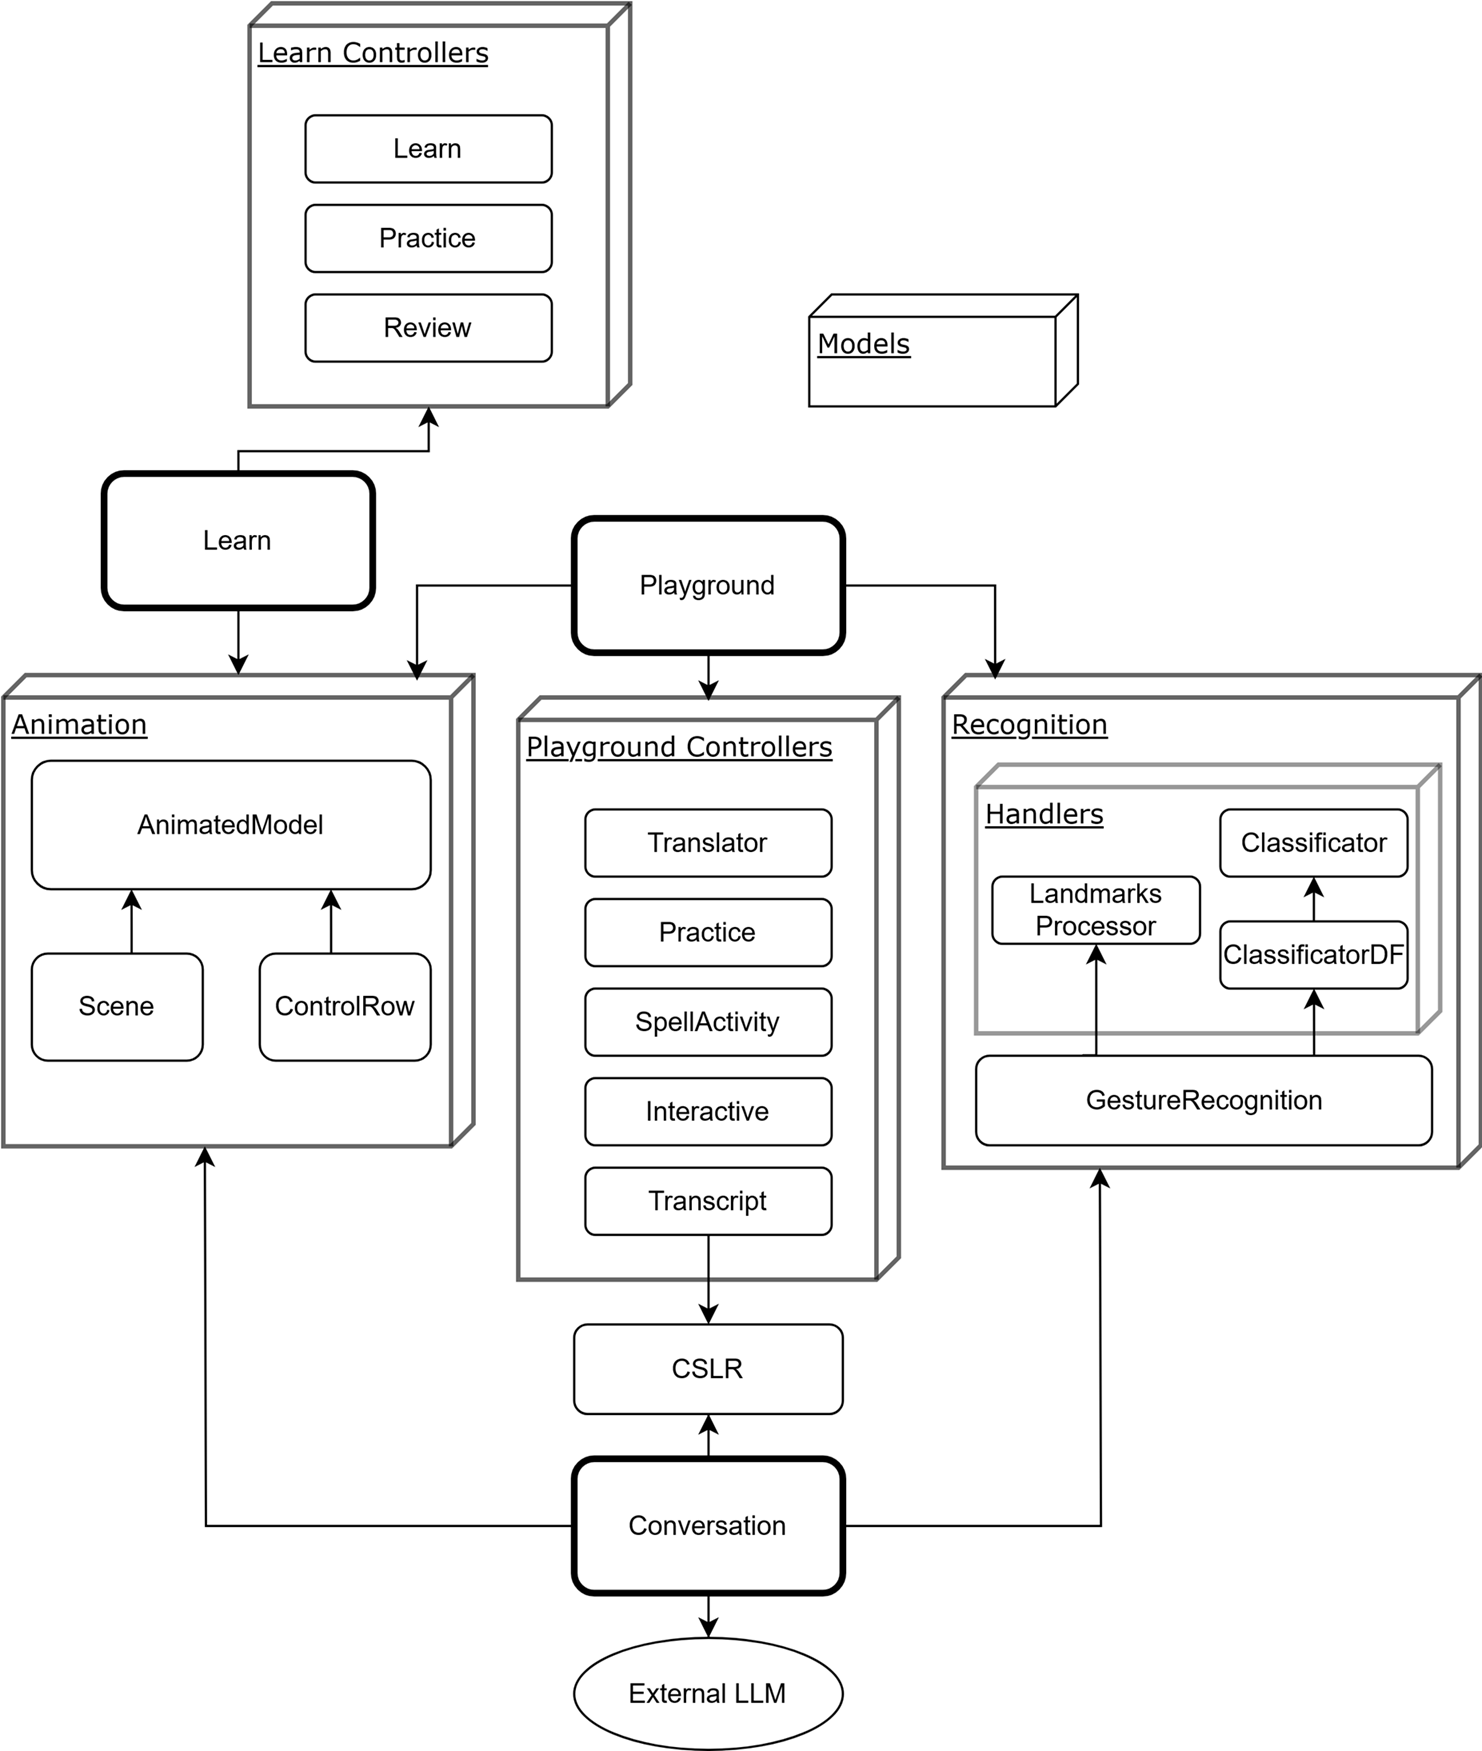
\includegraphics[width=1\columnwidth]{graphics/webapp-architecture-diagram.png}
            \caption{Diagram architektury celé aplikace}
            \label{webapp-architecture-diagram}
        \end{figure}
            

        \subsubsection{Podrobnější popis hlavních komponent a~architektury}
            V~aplikaci se nachází dvě hlavní komponenty. 
            \begin{itemize}
                \item AnimatedModel \par
                    Komponenta \emph{AnimatedModel} obsahuje logiku pro vykreslování 3D modelu a~pro řízení a~přehrávání animací. Tato komponenta se používá v~další komponentě \emph{Scene}, která definuje scénu, do které je model vykreslen. Ostatní stránky nebo komponenty poté mohou využívat komponentu \emph{Scene} pro snadné vložení 3D scény s~modelem. \emph{Scene} poskytuje ostatním komponentám instanci \emph{AnimatedModel}, kde lze pomocí definovaného rozhraní řídit chování modelu. Stěžejní funkcí komponenty \emph{AnimatedModel} je \emph{playAnimationForText(text, language)}, která pro zadaný text spustí sekvenci animací, znakující daný text v~zadaném jazyku.
    
                    Pomocí další komponenty \emph{ControlRow} lze přidat možnost ovládání animací. Tato komponenta umožňuje volbu rychlosti přehrávání animací a~možnost pozastavení celé animace.
    
                \item GestureRecognition \par
                    Druhou významnou komponentou je \emph{GestureRecognition}. Tato komponenta je zodpovědná za zobrazení záznamu webkamery, rozeznání souřadnic ruky pomocí MediaPipe frameworku, zpracování rozpoznaných souřadnic a~klasifikaci gest. Při použití této komponenty se lze přihlásit k~odběru zpráv, které obsahují pravděpodobnosti právě vyobrazeného znaku.

                    Logika zpracování rozpoznaných souřadnic ruky se nachází v~souboru \emph{LandmarksProcessor.ts}. Klasifikátor \emph{ClassificatorDF.ts} implementuje rozhraní \emph{Classificator.ts} a~je zodpovědný za klasifikaci zpracovaných souřadnic danou AI metodou.
            \end{itemize}

        Na stránce \emph{Cvičiště} je poté mezi tyto dvě komponenty vložena komponenta třetí -- Controller, řídící logiku zvoleného režimu. Každý režim má vlastní řídící komponentu, která zpracovává vstup od uživatele a~komunikuje s~\emph{AnimatedModel} a~\emph{GestureRecognition}. Stránka poskytuje Controller komponentám instanci komponenty \emph{AnimatedModel} pro umožnění řízení animací a~přeposílá jim zprávy o~rozpoznaných gestech.

        Stránka \emph{Učitel} je vytvořena obdobně. Stránka zobrazující animovaný model umožňuje přepínat mezi třemi Controller komponentami, které zpracovávají vstup uživatele a~komunikují s~poskytnutou instancí \emph{AnimatedModel}.

        Stránka \emph{Konverzace} je založena také na zmíněných hlavních komponentách. Tento režim je vytvořen na jedné stránce, která vykresluje uživatelské rozhraní a~řídí komunikaci mezi komponentami, vstupem uživatele a~rozhraním LLM modelů.

        Některé komponenty využívají stejné funkce jako ostatní. Tyto funkce jsou extrahovány do pomocných TypeScript souborů za účelem omezení duplikace stejného kódu a~oddělení zodpovědnosti. Zajímavou funkci lze například vidět v~souboru \emph{CSLR.ts}, jejíž účel je detailně popsán v~podkapitole \ref{cslr-text}.


    \subsection{Přehrávání animací a~zobrazení modelu v~Threlte}
        Tato podkapitola popisuje použití vytvořeného 3D modelu člověka, jeho vykreslení, animování a~řízení průběhu animace na webové stránce, konkrétně pomocí technologie Threlte.
        
        \subsubsection{Scéna}
            K~vyobrazení modelu je potřeba nejprve vytvořit scénu, ve které se bude model nacházet. Tato scéna se skládá z~osvětlení, kamery a~pozadí. Ve zdrojovém kódu se nachází komponenta \emph{Scene}, která definuje právě tuto scénu.
            Značkou \emph{<Canvas>} se definuje oblast, ve které se bude 3D grafika vykreslovat. Uvnitř oblasti se nachází \emph{<T.PerspectiveCamera>} a~\emph{<T.AmbientLight>}, které definují kameru a~osvětlení scény. Tato komponenta také obsahuje komponentu \emph{<T.OrbitControls>}, která umožňuje uživateli ovládat pohled kamery pomocí myši. Posledním objektem uvnitř scény je samotný model, který je zobrazen pomocí Svelte komponenty \emph{AnimatedModel}.

        \subsubsection{Vykreslení modelu}
            Komponenta \emph{AnimatedModel} obsahuje definici vykreslení modelu postavy a~algoritmus řídící přehrávání animací. Její základ je vygenerován na základě poskytnutého 3D modelu pomocí nástroje \emph{@threlte/gltf}. Obsahuje několik funkcí, kterými ji lze ovládat. Nejdůležitější funkcí je \emph{playAnimationForText(text, language)}, která spustí řízení sekvence animací odpovídající zadanému textu a~jazyku.

            K~načtení modelu nabízí Threlte funkci \emph{useGltf(model, options)}, pomocí které lze načíst model. V~options lze například nastavit využití Draco komprese.


        \subsubsection{Ovládání animací} \label{ovladani-animaci}
            K~animacím modelu se v~Threlte přistupuje pomocí actions a~mixer, které lze získat pomocí funkce \emph{useGltfAnimation(gltf, ref)}, kde \emph{gltf} je právě načtený model pomocí funkce \emph{useGltf}. Slovník \emph{actions} obsahuje všechny dostupné animace, ke kterým lze přistupovat pomocí klíče odpovídajícího názvu animace uvnitř 3D modelu. Animaci lze spustit pomocí nalezení v~kolekci \emph{actions} a~zavolání funkce \emph{play()} nad danou instancí.

            K~určení bodu začátku následující animace pro nadcházející znak je potřeba detekovat konec aktuální animace. Instance \emph{mixer} umožňuje odběr události, která je volána při ukončení animace.

            K~plynulému přechodu mezi animacemi slouží funkce \emph{transitionTo(action, duration)}. Tato funkce nastaví následující animaci a~nad aktuálně přehrávanou animací zavolá funkci \emph{crossFadeTo(action, duration)}, která plynule přejde z~jedné animace do druhé.


        \subsubsection{Ukázka kódu frameworku Threlte}
            Vytvoření scény, ve které se nachází 3D model postavy, lze vidět ve zdrojovém kódu \ref{threlte-code}.

            \begin{kicode}{JavaScript}{threlte-code}{Ukázka Threlte scény s~3D modelem, kamerou a~osvětlením}
const gltf = useGltf('models/Model.glb', {useDraco: true})

// Přehrávání animací
const { actions, mixer } = useGltfAnimations(gltf)

// Spustí animaci, když se změní hodnota currentActionName
$: $actions[currentActionName]?.play()

// Změna rychlosti přehrávané animace
mixer.timeScale = speed;

<Canvas>
    <T.PerspectiveCamera makeDefault position={[0, 0, 0.8]} fov={60}>
        <OrbitControls autoRotate={false} enableZoom={true} enableDamping={false} />
    </T.PerspectiveCamera>

    <T.AmbientLight intensity={5} />

    <T is={\$gltf.scene} position = {[0, -1.5, 0]} />
</Canvas>
            \end{kicode}


    
    \subsection{Rozpoznání gest ruky}
        K~rozpoznání gesta ruky na webové stránce je potřeba získat snímek z~webkamery. Na takovém snímku poté provést stejné rozpoznání a~zpracování souřadnic ruky jako při trénování z~datasetu a~následně výsledek klasifikovat pomocí vytvořeného klasifikátoru. 
        
        Celý proces rozpoznání je zobrazen na následujícím diagramu znázorněném na obrázku \ref{gesture-recognition-diagram}.

        \begin{figure}[htbp]
            \centering
            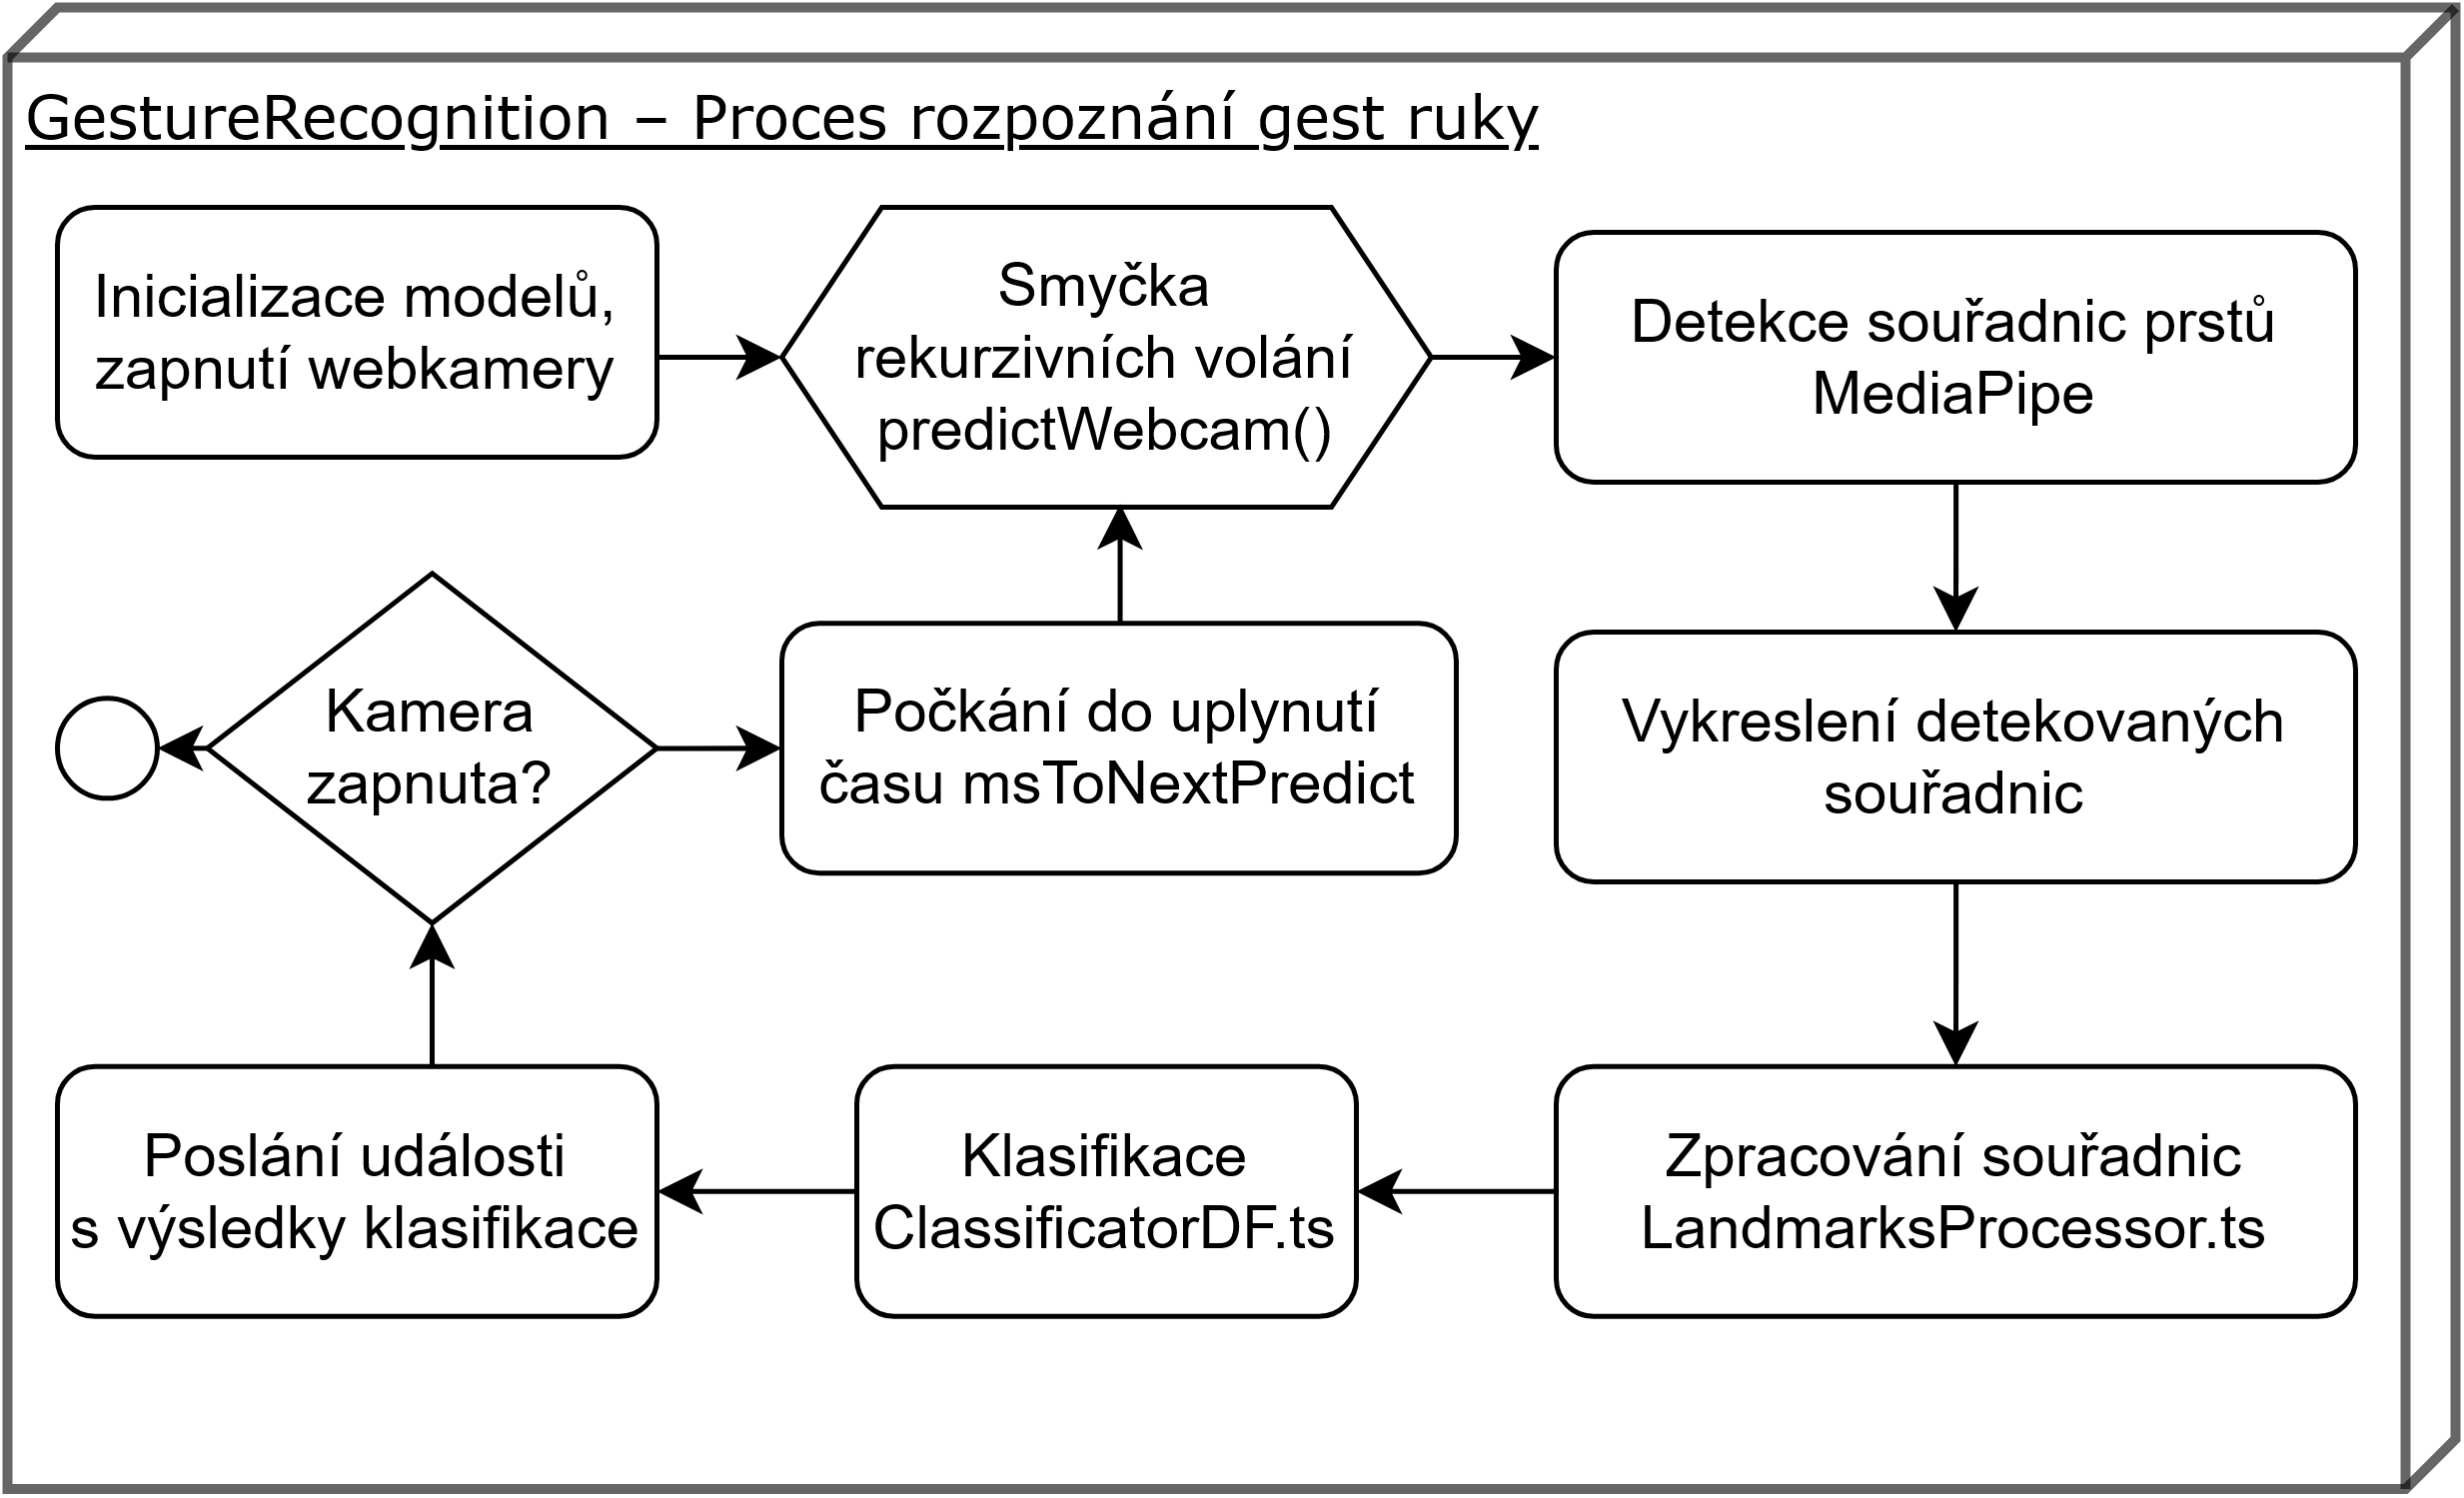
\includegraphics[width=0.8\columnwidth]{graphics/gesture-recognition-diagram.png}
            \caption{Diagram procesu rozpoznání gest ruky}
            \label{gesture-recognition-diagram}
        \end{figure}
        
    
        \subsubsection{Použití MediaPipe Solutions v~JavaScriptu}

            V~následujícím zdrojovém kódu \ref{mediapipe-javascript} lze vidět ukázku použití MediaPipe Solutions v~JavaScriptu. Funkce \emph{detectForVideo} rozpoznává souřadnice prstů ruky a~vrací 21 souřadnic při úspěšném rozpoznání.

        \begin{kicode}{JavaScript}{mediapipe-javascript}{Ukázka MediaPipe Solutions v~JavaScriptu}
import {HandLandmarker, FilesetResolver} from '@mediapipe/tasks-vision';

const vision = await FilesetResolver.forVisionTasks('wasm-taskvision');

handLandmarker = await HandLandmarker.createFromOptions(vision, {
    baseOptions: {
        modelAssetPath: `hand_landmarker.task`,
        delegate: 'GPU'
    },
    runningMode: 'VIDEO',
    numHands: 1
});

const results: HandLandmarkerResult = handLandmarker.detectForVideo(video, startTimeMs);
        \end{kicode}
        

    
        \subsubsection{Použití TensorFlow Decision Forests modelu v~JavaScriptu}
            Pomocí zmíněné knihovny TensorFlow.js se nejprve načte model klasifikátoru. Poté je nad instancí tohoto modelu volána funkce \emph{executeAsync}, jejímž vstupem jsou zpracované souřadnice ruky a~výstupem jsou pravděpodobnosti každého znaku na základě vstupu. Ukázku použití lze vidět ve zdrojovém kódu \ref{tfdf-javascript}.

            \begin{kicode}{JavaScript}{tfdf-javascript}{Ukázka TensorFlow.js}
import * as tf from '@tensorflow/tfjs-core';
import * as tfdf from '@tensorflow/tfjs-tfdf';
tfdf.setLocateFile(`inference.wasm`);

// Načtení modelu
model = await tfdf.loadTFDFModel("model.json");

// Klasifikace dat, kde tensor obsahuje zpracované souřadnice
const output = (await model.executeAsync(tensor)) as tf.Tensor;
            \end{kicode}

    
    \subsection{Rozhraní a~výkon aplikace}
        Rozhraní aplikace je responzivní, aplikaci lze používat jak na mobilním zařízení, tak i~na větším monitoru. Pro komfortní použití aplikace je potřeba stále vidět animaci, záznam kamery i~ovládací prvky, a~proto doporučuji používat aplikaci na zařízení s~větší obrazovkou.

        Zobrazení na menších obrazovkách využívá netradiční řešení. Místo zmenšení nebo změny uspořádání prvků aplikace využívá fixní pozicování. V~režimu \emph{Konverzace} je v~levém horním rohu okno webkamery a~v~pravém dolním rohu tlačítko pro odesílání zprávy. V~režimu \emph{Učitel} je animace v~levém dolním rohu obrazovky. Zmíněné prvky jsou ve fixních pozicích stále, nezávisle na aktuálně zobrazené části stránky. Tímto přístupem lze stále vidět podstatnou část stránky a~při tom využívat ovládací prvky, které by jinak na menších obrazovkách nebyly současně vidět. Obrázek \ref{mobile} zobrazuje vzhled aplikace na mobilním zařízení.

        Aplikace, obzvlášť v~režimech s~animací a~rozpoznáním zároveň, je znatelně náročná na systémové požadavky zařízení. Na průměrně výkonných telefonech může být přehrávání animací viditelně neplynulé, a~proto doporučuji aplikaci používat na počítačích. Na běžně výkonném počítači je aplikace zcela plynulá.

 %       Rychlost rozpoznávání gest lze rozdělit na dva úseky. Následující měření času bylo provedeno na moderním počítači a slouží zejména k porovnání poměru. Rozpoznání souřadnic ruky pomocí MediaPipe frameworku trvalo 6 ms. Klasifikace souřadnic se zpracováním souřadnic trvala 1-2 ms – zhruba třetinu času.


        \begin{figure}[H]
            \centering
            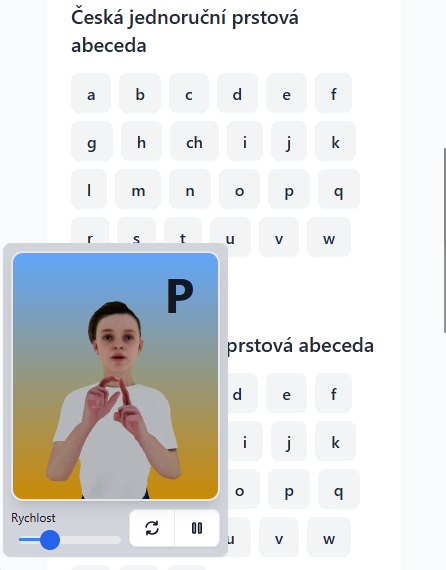
\includegraphics[width=0.5\columnwidth]{graphics/mobile.png}
            \caption{Webová aplikace na zařízení s~malou obrazovkou}
            \label{mobile}
        \end{figure}
        
        
    \subsection{Nasazení aplikace}
        Aplikace je určena pro provoz na webovém serveru Node.js. Pro jednoduché nasazení je k~dispozici \emph{Dockerfile}, který umožňuje spuštění aplikace v~Docker kontejneru.
        
        Při nasazení mimo lokální síť je nutné provozovat webovou aplikaci přes protokol \emph{https}, protože prohlížeče z~bezpečnostních důvodů blokují přístup k~webkameře při použití protokolu \emph{http}.
        
        Pro správné fungování aplikace v~režimu PWA je rovněž nutné, aby webový server disponoval platným SSL certifikátem.

\clearpage


\section{Uživatelská příručka webové aplikace}
    Tato kapitola popisuje jednotlivé funkční části aplikace z~hlediska jejich funkčnosti a~používání.

    \subsection{Obecné ovládání}
        V~následujících dvou podkapitolách je vysvětleno, jak uživatel může a~měl by přistupovat k~ovládání a~používání aplikace.
        
    \subsection{Ovládání kamery animace}
        Úhel přiblížení nebo pozici kamery lze v~animačním okně s~postavou ovládat. Držením levého tlačítka myši lze ovládat rotaci kamery. Pomocí pravého tlačítka lze pohybovat celou kamerou. Použitím kolečka lze měnit přiblížení.

        Rychlost přehrávání animace lze měnit posuvníkem pod oknem animace.

    \subsection{Ovládání rozpoznání prstové abecedy z~kamery}
        Ke správnému rozpoznávání znaků z~kamery je dobré vědět, jak aplikace uživatelovo znakování zaznamenává a~podle toho se přizpůsobit očekávanému chování uživatele ze strany aplikace.

        \subsubsection{Rozpoznání jednotlivých znaků}
            V~režimech, kde aplikace očekává jen jeden konkrétní znak, je použití intuitivní. Stačí daný znak zřetelně ukázat před kamerou a~aplikace jej zaznamená. Tento způsob chování se například nachází v~režimu \emph{Cvičiště~--~Znakování}, kde aplikace čeká na zobrazení následujícího znaku zatím nerozpoznané části slova.

        \subsubsection{Rozpoznání souvislého textu}
            Tyto režimy jsou náročnější, protože se snaží přepsat plynulou sekvenci znaků do navazující sekvence slov. Tento režim se nachází na stránce \emph{Cvičiště} v~režimu \emph{Přepis} a~na stránce \emph{Konverzace}. Pro úspěch je klíčové:
            
            \begin{itemize}
                \item Sledovat zpětnou vazbu \par
                    Vždy věnujte pozornost textovému poli, kde se zobrazuje rozpoznaný text. Aplikace potřebuje, abyste každý znak chvíli podrželi, než ho zaregistruje. Nepřecházejte na další písmeno, dokud neuvidíte, že se to aktuální objevilo v~textovém poli.
                
                \item Vytváření mezer \par
                Chcete-li ukončit slovo a~začít nové (vložit mezeru), musíte znak posledního písmena slova podržet znatelně déle než ostatní znaky. Aplikace delší zobrazení znaku interpretuje jako signál pro vložení mezery.
                
                \item Znakování stejného písmene vícekrát za sebou \par
                    Tato situace vyžaduje specifický postup, protože aplikace nezaregistruje stejné písmeno dvakrát, při delším podržení daného znaku.
                    
                    \begin{itemize}
                        \item Ukažte znak písmena a~počkejte, až jej aplikace zapíše (uvidíte písmeno v~textovém poli).
                        \item Okamžitě poté, co se písmeno zapíše, krátce změňte gesto ruky. Nejjednodušší je ruku na chvíli uvolnit do neutrální polohy.
                        \item Poté znovu ukažte stejné písmeno, které chcete zapsat podruhé.
                    \end{itemize}

                    Pokud uživatel neuvolní ruku mezi stejným znakem dostatečně rychle, dojde k~rozeznání mezery. Pokud uživatel uvolní ruku na příliš dlouho, může dojít k~zapsání jiného znaku.
            \end{itemize}

    
    \subsection{Cvičiště}
        Stránka \emph{Cvičiště} slouží jako prostředí, ve kterém si uživatel může vyzkoušet různé režimy ve volnější formě než u~ostatních stránek. Uživatel má na výběr z~pěti režimů. Režimy \emph{Překladač} a~\emph{Odezírání} nevyžadují použití webkamery. Zbývající tři režimy \emph{Znakování}, \emph{Přepis} a~\emph{Procvičování} vyžadují pro svou funkčnost záznam webkamery. Vzhled stránky lze vidět na obrázku \ref{playground}.

        \begin{figure}[htbp]
            \centering
            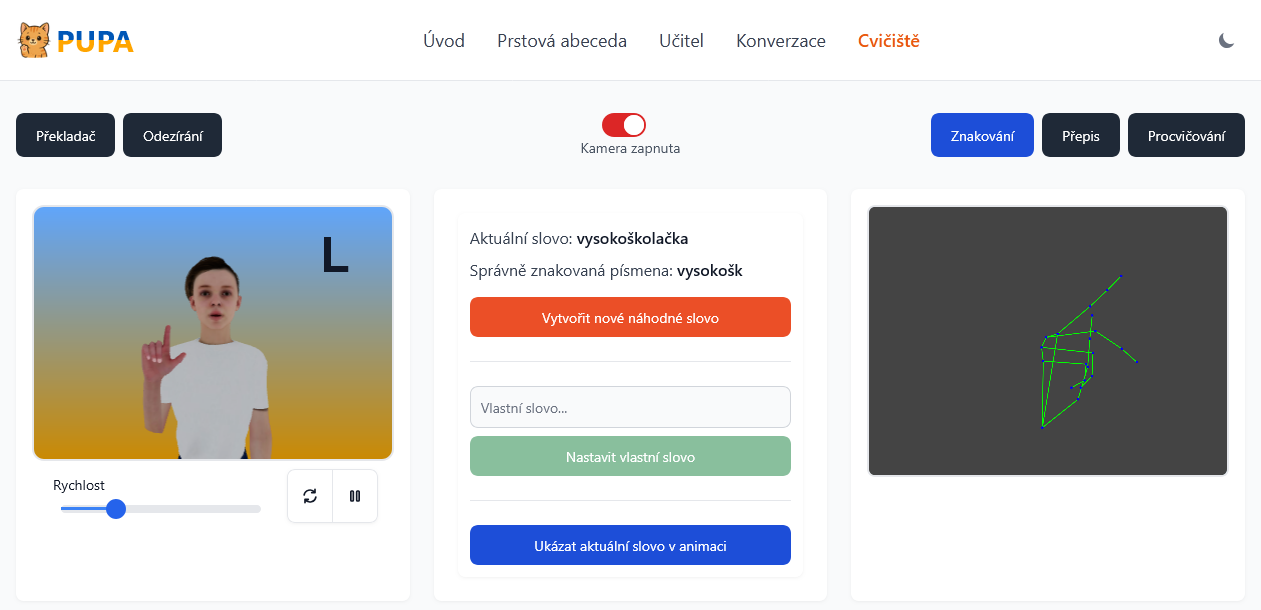
\includegraphics[width=1\columnwidth]{graphics/playground.png}
            \caption{Webová aplikace~--~Stránka Cvičiště}
            \label{playground}
        \end{figure}

        
        \subsubsection{Překladač}
            \emph{Překladač} slouží k~překladu textu do sekvence animací odpovídající zadanému textu a~jazyku. Uživatel si může vybrat z~jednoruční nebo dvouruční prstové abecedy a~českého znakového jazyka. Volba znakového jazyka přehraje znak slova, pokud pro něj existuje animace. Pokud pro daný znak animace neexistuje, model zobrazí dané slovo v~jednoruční prstové abecedě.

        \subsubsection{Odezírání}
            \emph{Odezírání} je režim, ve kterém je uživateli ukázáno náhodné slovo v~podobě animace a~uživatel má za úkol dané slovo rozpoznat a~zapsat. Aplikace poté zkontroluje, zda zadané slovo odpovídá náhodně zvolenému slovu. 
            
            Aplikace obsahuje zhruba 23000 náhodných českých slov \cite{ceska-slova}. Při volbě znakového jazyka se slova generují stále stejným způsobem a~je tedy pravděpodobné, že pro dané slovo nebude existovat animace. Pro procvičování znakového jazyka pouze s~existujícími animacemi může uživatel využít procvičení na stránce \emph{Učitel}.
        
        \subsubsection{Znakování}
            Tento režim slouží pro procvičení znakování. Uživatel si může vymyslet své vlastní slovo, nebo si jej může vygenerovat jako v~režimu \emph{Odezírání}. Rozdílem oproti předchozímu režimu ale je, že uživatel má nyní dané slovo ukázat před webkamerou. Webová aplikace přitom kontroluje, zda uživatel dané slovo znakuje správně. Pokud uživatel nebude vědět, jak dané slovo znakovat, může si slovo přehrát v~animaci stiskem tlačítka.
        
        \subsubsection{Přepis}
            Režim \emph{Přepis} má dvě volby~--~\emph{Automatický} a~\emph{Manuální}. V~automatickém režimu aplikace rozpoznává znaky, které uživatel ukazuje před webkamerou, a~aplikace se snaží přepsat sekvenci rozpoznání do věty. V~manuálním režimu namísto automatického zaznamenávání musí uživatel manuálně potvrdit zaznamenání aktuálně ukázaného znaku.
        
        \subsubsection{Procvičování}
            \emph{Procvičování} na stránce \emph{Cvičiště} je nejinteraktivnějším režimem. Uživatel si zde může vymyslet vlastní text, který poté střídavě znakuje spolu s~animací. 
            
            Každý znak nejprve ukáže model v~animaci a~poté musí uživatel zobrazený znak zobrazit správně před webkamerou. Až po úspěšném zobrazení dochází k~přechodu k~dalšímu znaku. Cíl uživatele je takto projít celým textem.
        
    \subsection{Učitel}
        Stránka \emph{Učitel} provádí uživatele postupně všemi znaky jazyka. Nabízí českou jednoruční a~dvouruční prstovou abecedu a~také český znakový jazyk. Tento režim lze rozdělit na tři části~--~\emph{Procvičovat}, \emph{Učit} a~\emph{Znaky}. Vzhled stránky lze vidět na obrázku \ref{ucitel}.

         \begin{figure}[htbp]
                \centering
                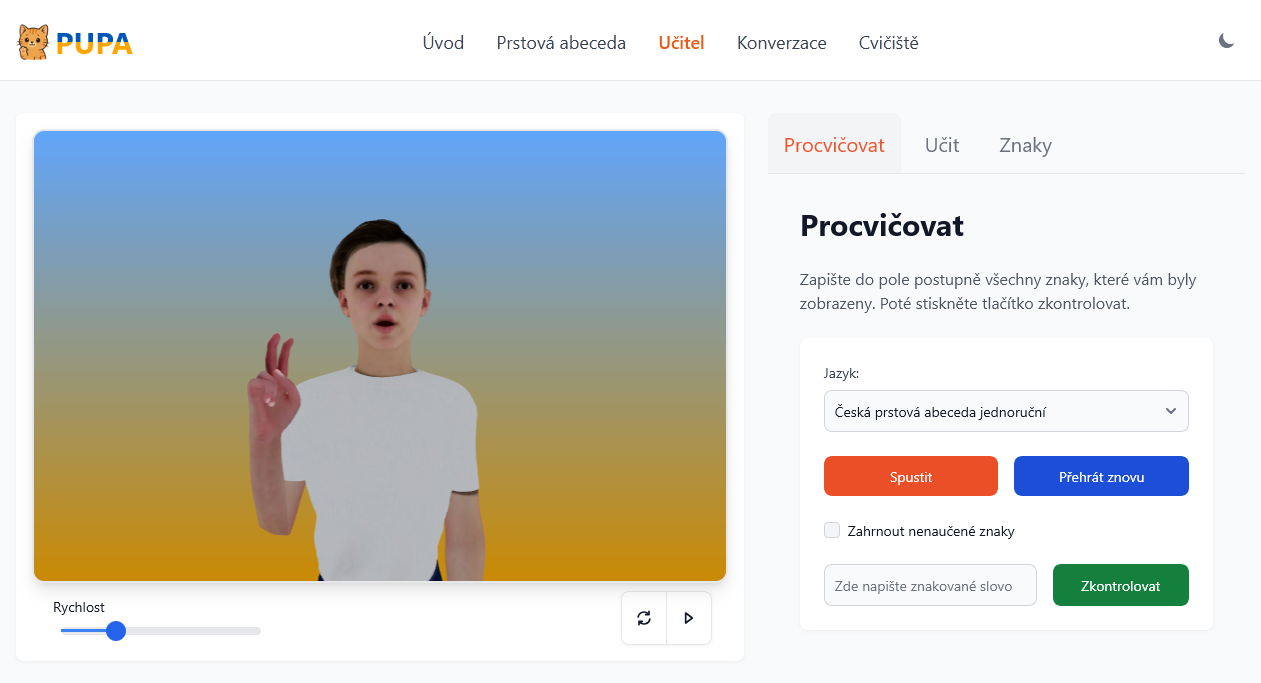
\includegraphics[width=1\columnwidth]{graphics/ucitel.png}
                \caption{Webová aplikace~--~Učitel}
                \label{ucitel}
            \end{figure}

        \subsubsection{Procvičovat}
            Režim \emph{Procvičovat} slouží k~procvičování již naučených znaků. Aplikace náhodně vygeneruje jeden z~naučených znaků a~přehraje jej v~rámci okna animace. Uživatel poté musí daný znak rozeznat a~zapsat. Uživatel může svou odpověď zkontrolovat a~případně daný znak přehrát znovu.

        \subsubsection{Učit}
            Učení nových znaků probíhá v~režimu \emph{Učit}. Zde je uživateli přehrán následující, zatím nenaučený, znak v~animaci. Uživatel si může danou animaci přehrát vícekrát a~rozhodnout se, že si přehrávaný znak již pamatuje a~označit jej za naučený.

        \subsubsection{Znaky}
            V~režimu \emph{Znaky} lze sledovat aktuální postup již naučených znaků. Lze si zde všechny znaky přehrávat a~také je lze zrychleně označit za již naučené dvojitým kliknutím.

    \subsection{Konverzace} \label{up-konverzace}
        Stránka \emph{Konverzace} poskytuje nejinteraktivnější možnost procvičování prstové abecedy. Stránka se skládá ze tří hlavních částí. Uprostřed obrazovky se nachází 3D model, se kterým uživatel komunikuje. V~levé části lze vidět záznam webkamery a~také ovládací prvky. V~pravé části se nachází historie konverzace. Režim je založen na konverzaci, kde uživatel komunikuje s~modelem prostřednictvím české jednoruční prstové abecedy. Uživatel nejdříve vyznakuje sekvenci znaků, která je převedena do věty. Tato věta je odeslána nastavenému LLM modelu a~odpověď tohoto modelu je uživateli prezentována v~podobě animace.


        Velkou výhodou použití velkých jazykových modelů je jejich schopnost pochopení textu s~chybami. Díky této vlastnosti nemusí uživatel cílit na zcela správně rozpoznaný text a~může pokračovat ve znakování dále, ačkoliv systém rozpoznal některý z~předchozích znaků špatně, nebo se v~něm uživatel spletl.

        Rozhraní stránky \emph{Konverzace} lze vidět na obrázku \ref{konverzace}.

         \begin{figure}[htbp]
                \centering
                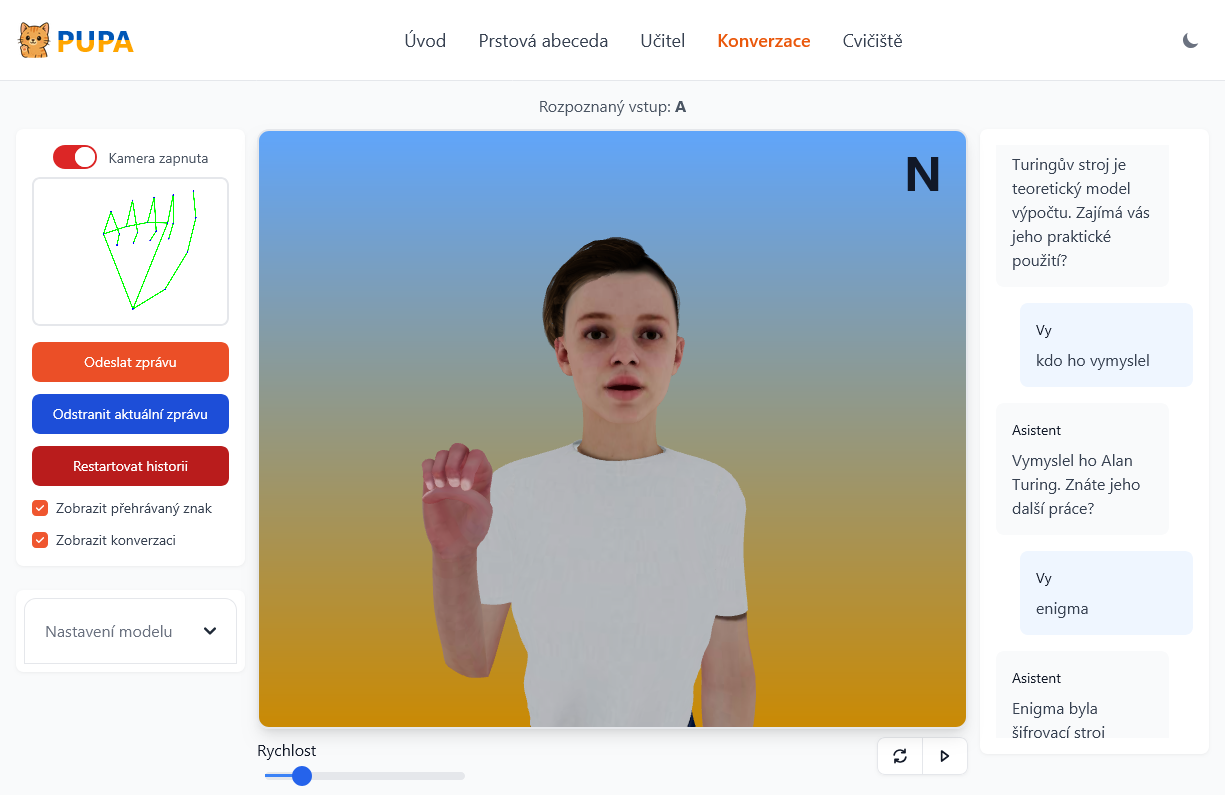
\includegraphics[width=1\columnwidth]{graphics/konverzace.png}
                \caption{Webová aplikace~--~Konverzace}
                \label{konverzace}
            \end{figure}

        \subsubsection{Nastavení LLM}
            Aplikace podporuje dvě rozhraní pro komunikaci s~LLM modelem. Prvním z~nich je \emph{ollama}~--~populární nástroj pro spouštění jazykových modelů \cite{ollama} a~druhým rozhraním je \emph{platforma OpenAI} \cite{open-ai}. Aplikace obsahuje pole pro nastavení komunikace mezi těmito rozhraními, avšak pokud by uživatel chtěl použít rozhraní jiné, nic mu nebrání ve vytvoření vlastního překladače dotazů mezi webovou aplikací a~zvoleným modelem.
        
        \subsubsection{Ollama}
                Nejdříve je potřeba nainstalovat program ollama, nastavit CORS pro povolení cross-origin mezi webovou aplikací a~programem ollama. Posledním krokem je instalace některého modelu a~jeho spuštění.
                
                Webová aplikace má již přednastavenou výchozí adresu programu a~stačí pouze změnit název modelu na ten, který si uživatel nainstaloval a~spustil.


                Postup instalace ollama na vlastním počítači popisuje následující seznam kroků.

                \begin{enumerate}
                    \item \emph{Instalace programu ollama} \par
                        Stáhnutí instalačního balíčku na adrese: \emph{ollama.com/download} a~jeho nainstalování.
                    \item \emph{Povolení CORS} \par
                        Nastavení proměnné prostředí \emph{OLLAMA\_ORIGINS = adresa\_aplikace} a~restartování programu ollama.
                        Například v~operačním systému Windows stačí v~příkazové řádce zadat: \\\emph{'SET OLLAMA\_ORIGINS = https://158.194.92.104'}.
                        
                    \item \emph{Stažení modelu} \par
                        Vybrání modelu na adrese: \emph{ollama.com/search} a~jeho stažení pomocí příkazu \emph{ollama run název\_modelu}. 
                        Před vybráním modelu je potřeba se zamyslet nad jeho velikostí. Velikost modelu by neměla přesahovat velikost volné operační paměti, případně velikost paměti grafické karty.
                        
                    \item \emph{Spuštění modelu} \par
                        Již stažený model lze zapnout stejným příkazem: \\\emph{ollama run název\_modelu}.
                        
                    \item \emph{Ukončení modelu} \par
                        Pro vypnutí modelu a~uvolnění paměti stačí napsat do příkazové řádky s~běžícím model příkaz \emph{/bye}.
                \end{enumerate}

            \subsubsection{OpenAI}
                Pro komunikaci přes rozhraní společnosti OpenAI je nejprve potřeba získat API klíč. Ten lze získat na platformě zmíněné společnosti, ke~které lze přistoupit na adrese: \emph{platform.openai.com}. Tento přístup je placený, ale značně ulehčuje zprovoznění režimu a~také nabízí řádově rychlejší a~větší modely, které nelze spustit na běžném počítači. Zmíněné větší modely poskytují přesnější odpovědi a~díky tomu dokážou vést zajímavější a~zábavnější konverzaci s~uživatelem. Uživatel v~nastavení aplikace pouze vloží svůj API klíč a~název vybraného modelu a~může režim plně využívat.
        
        \subsubsection{Klávesové zkratky}
            Uživatel může využívat klávesy \emph{Mezerník} pro vytvoření mezery v~aktuálním místě vstupu a~také \emph{Backspace} pro smazání posledně zaznamenaného znaku. Klávesa \emph{Enter} odešle aktuální zprávu.

    \subsection{Používání aplikace bez internetu}
        Vytvořená webová aplikace je PWA aplikací~--~progressive web application. Umožňuje instalaci na uživatelovo zařízení a~nainstalovanou aplikaci lze poté používat bez přístupu k~internetu. Nainstalovanou aplikaci lze ale také samozřejmě používat i~s~připojením k~internetu a~využívat \emph{OpenAI API} na stránce \emph{Konverzace}.
        
        V~desktopovém prohlížeči lze aplikaci nainstalovat pomocí otevření webové aplikace v~prohlížeči a~stisknutí ikony zobrazené v~pravém okraji adresního řádku prohlížeče.

        Na mobilním zařízení lze stránku nainstalovat pomocí otevření stránky v~prohlížeči a~zvolení položky \emph{Přidat na domovskou obrazovku}, která po stisknutí nabídne instalaci aplikace.

        Instalace byla otestována a~je funkční v~prohlížeči \emph{Google Chrome}. Nainstalovaná aplikace nabízí všechny funkcionality jako při používání ve webovém prohlížeči.

\clearpage



\section{Rozšíření}
    V~této kapitole budou probrána některá z~možných a~vhodných rozšíření aplikace. Tato rozšíření nejsou implementována. Zde je pouze zmíněn možný přístup k~jejich řešení a~zdůvodnění jejich významu.

%(todo) rozšíření možných řešení problémů transformery atd.

    \subsection{Implementace pro znakový jazyk}
        Aplikace je lehce rozšířitelná tak, aby podporovala slova ze znakového jazyka, ale není v~ní tento režim znatelně zastoupen z~důvodu náročnosti tvorby animací.
            
        \subsubsection{Animace a~snímání pohybu}
            Zajímavým přístupem, jak efektivně animovat 3D model člověka, je snímání pohybu (anglicky motion capture). Zjednodušeně si lze tuto metodu představit tak, že počítač pohybuje s~3D modelem člověka podle reálné předlohy. Problém nastává s~přesností zaznamenávání pohybu. Motion capture je velmi využíván ve tvorbě filmů a~her, kde herci využívají speciálních nástrojů, které dokážou snímat jejich pohyb velice přesně. Dostupnějším řešením je použití kamery, pomocí které lze rozpoznávat souřadnice specifických částí těla, podobně jako použitý model na rozpoznání souřadnic ruky v~této práci. Volně dostupné programy převádějící vstup kamery na animace se ukázaly jako nedostatečně přesné.
            
        
        \subsubsection{Rozpoznání}
            Znaky slov jsou mnohem komplexnější oproti znakům prstové abecedy. Jejich rozpoznání by vyžadovalo použití rozpoznání prstů a~postavy. Použitý framework MediaPipe obsahuje Holistic Landmarker, který kombinuje modely pro rozpoznání obličeje, postavy a~prstů. Na základě těchto dat by bylo možné natrénovat model obdobně jako při rozpoznávání prstové abecedy. Nicméně takový model by nebyl dostatečný, jelikož mnoho znaků nemá statickou reprezentaci, ale vyžadují souvislý pohyb. Na tento problém lze narazit i~u~prstové abecedy.
            
     
    \subsection{Rozpoznání pohyblivých gest}
        Některé znaky jsou založeny nejen na statické pozici prstů, ale také na pohybu ruky. Příkladem může být písmeno J, jehož znak kombinuje pohyb ruky spolu s~pozicí prstů, nebo čárky a~háčky, které jsou také znakovány pomocí pohybu ruky. Tyto pohyby ale nejsou detekovány použitou metodou rozpoznávání a~také nebyla probrána možná řešení tohoto problému. Tímto problémem jsem se nezabýval, protože zobrazení háčku a~čárek není složité a~z~mého pohledu by dané rozpoznávání neúměrně celý proces ztížilo.

\clearpage


\begin{kiconclusions}
    Práce se zabývá vývojem webové aplikace pro podporu výuky české jednoruční prstové abecedy. Aplikace integruje převod textu na 3D animaci a~rozpoznávání znaků z~videozáznamu, čímž vytváří komplexní prostředí pro efektivní učení a~procvičování prstové abecedy.

    Proces převodu textu na animaci vychází z~předem vytvořeného 3D modelu postavy. Pro tento model byly vytvořeny animace české jednoruční i~dvouruční prstové abecedy včetně reprezentace diakritiky a~také animace několika základních slov českého znakového jazyka. Tento model je následně vykreslován ve webovém prohlížeči pomocí knihovny Three.js a~nabízí uživateli možnosti měnit rychlost přehrávání animace či ovládat pohled kamery.
    
    Rozpoznávání prstové abecedy ze záznamu webkamery bylo implementováno pro českou jednoruční prstovou abecedu. Aplikace je schopna spolehlivě rozpoznávat znaky zobrazované uživatelem. Tato funkce je v~aplikaci využita dvěma hlavními způsoby: zaprvé slouží k~ověření správnosti zobrazeného znaku, zadruhé umožňuje pokus o~přepis souvislé sekvence znakování do souvislé textové podoby pomocí vyvinutého heuristického algoritmu.
    
    Samotný proces rozpoznání gesta je dvoufázový. Nejprve jsou extrahovány souřadnice klíčových bodů ruky pomocí modelu Hand Landmark Detection z~frameworku MediaPipe Solutions, který poskytuje robustní a~přesnou detekci. Následně jsou tyto souřadnice transformovány a~klasifikovány modelem typu Gradient Boosted Trees, natrénovaným s~využitím knihovny TensorFlow. Trénovací dataset pro tento model obsahuje 7217 snímků od dvou osob a~byl vytvořen v~rámci této práce.
    
    Spojením těchto dvou klíčových funkcionalit vznikla webová aplikace postavená na frameworku SvelteKit. Aplikace integruje zmíněné technologie a~vytváří tak interaktivní prostředí pro výuku české prstové abecedy. Nabízí několik režimů použití: volnější režim Cvičiště pro experimentování, strukturovanější režim Učitel pro systematickou výuku a~inovativní režim Konverzace, ve kterém může uživatel oboustranně komunikovat s~velkým jazykovým modelem prostřednictvím znakování české jednoruční prstové abecedy.
    
    I~přes možná další rozšíření je výsledná aplikace plně funkční a~představuje cennou pomůcku pro výuku. Zejména režim konverzace se ukázal jako zajímavý a~zábavný způsob procvičování, který může významně přispět k~osvojení prstové abecedy. Navíc implementace české dvouruční prstové abecedy a~snadná rozšiřitelnost pro znaky znakového jazyka otevírají dveře k~dalšímu rozvoji aplikace.
\end{kiconclusions}

\begin{kiconclusions}[english]
    This thesis addresses the development of a web application to support the learning of the Czech one-handed finger alphabet. The application integrates text-to-3D animation conversion and finger alphabet recognition from video recordings, creating a comprehensive environment for effective learning and practicing the finger alphabet.

    The text-to-animation conversion process is based on a pre-existing 3D character model. For this model, animations were created for the Czech one-handed and two-handed finger alphabets, including the representation of diacritics, as well as animations for a few basic words of Czech Sign Language. This model is subsequently rendered in a web browser using the Three.js library and offers the user the options to change the animation playback speed or control the camera view.
    
    Finger alphabet recognition from webcam recordings was implemented for the Czech one-handed finger alphabet. The application is able to reliably recognize signs displayed by the user. This functionality is used in the application in two main ways: firstly, it serves to verify the correctness of the displayed sign and secondly, it allows attempting the transcription of a continuous sequence of signing into continuous text form using the developed heuristic algorithm.
    
    The gesture recognition process itself is two-phase. First, the coordinates of key hand landmarks are extracted using the Hand Landmark Detection model from the MediaPipe Solutions framework, which provides robust and accurate detection. Then these coordinates are transformed and classified by a Gradient Boosted Trees model, trained using the TensorFlow library. The training dataset for this model, containing 7,217 images from two individuals, was created as part of this work.
    
    Combining these two key functionalities resulted in a web application built on the SvelteKit framework. The application integrates the mentioned technologies, thus creating an interactive environment for learning the Czech finger alphabet. It offers several modes of use: a freer Playground mode for experimentation, a more structured Teacher mode for systematic learning, and an innovative Conversation mode in which the user can interact with a large language model through signing the Czech one-handed finger alphabet.
    
    Despite possible further expansions, the resulting application is fully functional and represents a valuable aid for learning. In particular, the conversation mode proved to be an interesting and entertaining method of practice, which can significantly contribute to the acquisition of the finger alphabet. Additionally, the implementation of the Czech two-handed finger alphabet and the easy extensibility for sign language signs open the door to further development of the application.
\end{kiconclusions}

\appendix


\section{Obsah přiloženého datového média} \label{sec:ObsahData}

\begin{description}

    \item[\texttt{text/}] \hfill \\
        Text práce a~veškeré soubory sloužící k~jeho vytvoření.
    
    \item[\texttt{src/}] \hfill \\
        Zdrojové kódy aplikace.
    
    \item[\texttt{dataset/}] \hfill \\
        Vytvořený dataset české jednoruční prstové abecedy.
    
    \item[\texttt{3D/}] \hfill \\
        Blender model obsahující vytvořené animace.
    
    \item[\texttt{README.txt}] \hfill \\ 
        Návod pro~zprovoznění aplikace.
   

\end{description}

%% Sazba volitelného seznamu zkratek, za~přílohami.
% \printglossary

\nocite{*}
\printbibliography

\end{document}